% !TEX program = pdflatex
% !TEX enableSynctex = true
\documentclass[aspectratio=169,10pt]{beamer}

%%%%%%%%%%%%%%%
\usepackage{booktabs}
\usepackage{xspace}
\usepackage{ulem}
\usepackage{subfig}
\usepackage{graphicx}
\usepackage{multirow}
\usepackage[capitalise,noabbrev]{cleveref} 
\usepackage{datatool}
\usepackage{algorithm} 
\usepackage{algpseudocode} 
\usepackage{empheq}
\usepackage[many]{tcolorbox}
\usepackage[capitalise,noabbrev]{cleveref}
\usetheme[progressbar=frametitle,block=fill]{metropolis}

\newcommand{\themename}{\textbf{\textsc{metropolis}}\xspace}
\definecolor{emphcolorval}{rgb}{0.23,0.4,0.7}
\definecolor{highlightcolorval}{rgb}{1,0,0}
% Penn colors
\definecolor{PennRed}{RGB}{149, 0, 26}
\definecolor{PennBlue}{RGB}{1, 37, 110}

\setbeamercolor{frametitle}{bg=PennBlue}
\setbeamercolor{progress bar}{fg=PennBlue}
\setbeamercolor{math text}{fg=PennRed}

\setbeamercolor{block title}{fg=PennBlue}
\setbeamercolor{block body}{fg=PennBlue}

\setbeamercolor{block title example}{fg=PennBlue}
\setbeamercolor{block body example}{fg=PennBlue, bg=yellow}

\setbeamersize{text margin left=5.5pt, text margin right=5.5pt}

\definecolor{cosmiclatte}{rgb}{1.0, 0.99, 0.95}
\setbeamercolor{background canvas}{bg=cosmiclatte}

\newcommand{\emphcolor}[1]{\textbf{\textcolor{emphcolorval}{#1}}}
%\newcommand{\mathcolor}[1]{{\mathbf{\color{emphcolorval}{#1}}}}
\newcommand{\highlightcolor}[1]{{\textbf{\color{highlightcolorval}{#1}}}}

% \usepackage{natbib}
% \bibliographystyle{ecta}

\crefname{equation}{}{}

\newtheorem{proposition}{Proposition}
\newcommand\bigzero{\makebox(0,0){\text{\huge0}}}
\newcommand{\D}[1][]{\ensuremath{\boldsymbol{\partial}_{#1}}}
\newcommand{\R}{\ensuremath{\mathbb{R}}}
\newcommand{\diff}{\ensuremath{\mathrm{d}}}
\newcommand{\ex}{\ensuremath{\mathrm{ex}}}
\newcommand{\set}[1]{\ensuremath{\left\{{#1}\right\}}}
\newcommand{\indicator}[1]{\ensuremath{\mathds{1}\left\{{#1}\right\}}}
\newcommand{\condexpec}[3][]{\ensuremath{\mathbb{E}_{#1}\left[{#2} \; \middle| \; {#3} \right]}}
\newcommand{\prob}[2][]{\ensuremath{\mathbb{P}_{#1}\left( {#2} \right)}}
\newcommand{\cprob}[2]{\ensuremath{\mathbb{P}\left( {#1}\left| {#2} \right. \right)}}
\newcommand{\condcov}[2]{\ensuremath{\mathrm{cov}\left({#1} \; \middle| \; {#2} \right)}}
\newcommand{\expec}[2][]{\ensuremath{\mathbb{E}_{{#1}}\left[ {#2} \right]}}
\newcommand{\bigO}[1]{\ensuremath{\mathcal{O}(#1)}}
\newcommand{\Xdom}{\mathcal{X}}
\newcommand{\Yrange}{\mathcal{Y}}
\newcommand{\Xtrain}{\hat{\mathcal{X}}}
\newcommand{\Xextr}{\mathcal{X}_{\mathrm{extr}}}
\newcommand{\Xhull}{\mathrm{Hull}(\Xtrain)}
\newcommand{\Xtest}{\mathcal{X}_{\mathrm{test}}}
\newcommand{\Ltest}{\ell_{\mathrm{test}}}
\newcommand{\F}{\mathcal{F}}
\newcommand{\Resid}{\mathcal{R}}
\newcommand{\st}{\textrm{s.t.}\,}
\newcommand\blfootnote[1]{%
	\begingroup
	\renewcommand\thefootnote{}\footnote{#1}%
	\addtocounter{footnote}{-1}%
	\endgroup
}
\newcommand{\loadmap}[2][map]{
	\DTLloaddb{#1}{#2}%
	\DTLforeach{#1}{\Key=Key,\Value=Value}{%
		\expandafter\def\csname#1\Key\expandafter\endcsname\expandafter{\Value}%
	}%
}
\newcommand{\mapvar}[2][map]{\csname #1#2\endcsname}

\loadmap{./figures/tex_parameter_map.csv} %loads map of parameters for direct insertion into the document.
\begin{document}
%\title{{\vspace{0.4in}\hspace{0.2in}\textcolor{PennBlue}{Spooky Boundaries at a Distance:\\\hspace{0.12in} Exploring Transversality and Stationarity with Deep Learning}}}
%\author{\hspace{0.2in}Mahdi Ebrahimi Kahou\inst{1}\and
%	Jes\'{u}s Fern\'{a}ndez-Villaverde\inst{2} \and Sebasti\'an G\'omez-Cardona\inst{1} \and Jesse Perla\inst{1} \and Jan Rosa\inst{1}}
%\institute{\inst{\hspace{0.2in}1}University of British Columbia,  Vancouver School of Economics\and
%	\inst{\hspace{0.2in}2}University of Pennsylvania}
%\date{\hspace{0.2in}\today }
%\maketitle
	
	
\title{{\vspace{0.4in}\hspace{0.0in}\textcolor{PennBlue}{Solving Equilibrium Models with \\ Modern Machine Learning Methods}}}
\author{\hspace{0.2in}Mahdi Ebrahimi Kahou\inst{1}}
\institute{\inst{\hspace{0.2in}1}University of British Columbia,  Vancouver School of Economics}
\date{\hspace{0.2in}\today }
\maketitle


\begin{frame}{Articles}
	\begin{itemize}
			\item \emphcolor{Exploiting Symmetry in High-Dimensional Dynamic Programming:} {\small with Jes\'{u}s Fern\'{a}ndez-Villaverde, Jesse Perla, and Arnav Sood}.\\ \medskip
			\item \emphcolor{Spooky Boundaries at a Distance: Exploring Transversality and Stability with Deep Learning:}  {\small with Jes\'{u}s Fern\'{a}ndez-Villaverde, Sebasti\'an G\'omez-Cardona, Jesse Perla, and Jan Rosa}.\\ \medskip
			\item \emphcolor{Are Minimizing the Euler and Bellman Residuals Enough?}
			
	\end{itemize}

\end{frame}


\section{\textcolor{PennBlue}{Background: Deep learning for functional equations}}

\begin{frame}
	\frametitle{Equilibrium conditions as functional equations}
	Most theoretical models in economics with equilibrium conditions can be written as functional equations:
	\begin{itemize}
		\item Take some function(s) $\psi \in \varPsi$ where $\psi : \Xdom\to \Yrange$ (e.g. asset price, investment choice, best-response).\vspace{0.1in}
		\item Domain $\Xdom$ could be state (e.g. dividends, capital, opponents state) or time if sequential.\vspace{0.1in}
		\item The ``model'' is $\ell: \varPsi \times \Xdom \rightarrow \Resid$ (e.g., Euler and Bellman residuals, equilibrium FOCs).\vspace{0.1in}
		\item The solution is the root of the model (residuals operator), i.e., $\mathbf{0} \in \Resid$, at each $x \in \Xdom$.\vspace{0.1in}
	\end{itemize}
	Then a \emphcolor{solution} is a $\psi^*\in \varPsi$ where $\ell(\psi^*,x) = 0$ for all $x \in \Xdom$.  How do we find an approximate solution?\vspace{0.1in}
\end{frame}

\begin{frame}
	\frametitle{Example: recursive formulation of the neoclassical growth}
	An example of a recursive case:
	\begin{itemize}
		\item Domain: $x = \begin{bmatrix*}
			k
		\end{bmatrix*}
		$ and $\Xdom = \R_+$.\vspace{0.1in}
		\item Solve for the optimal policy $k'(\cdot)$ and consumption function $c(\cdot)$: So $\psi : \R \to \R^2$ and $\Yrange = \R^2_+$.\vspace{0.1in}
		\item  Residuals are the Euler equation and feasibility condition, so $\Resid = \R^2$:
		\begin{align*}
			\ell(\underbrace{\begin{bmatrix*}k'(\cdot) & c(\cdot)\end{bmatrix*}}_{\equiv \psi}, \underbrace{k}_{\equiv x}) =
			\underbrace{\begin{bmatrix*}
					u'(c(k)) - \beta u'(c(k'(k)))\left(f'(k'(k)) + 1-\delta\right) \\
					f(k) - c(k) - k'(k) + (1-\delta)k
			\end{bmatrix*}}_{\text{model}}
		\end{align*}
		\item Finally,  $\psi^* = \left[k'(\cdot),c(\cdot)\right]$ is a solution if it has zero residuals on domain $\Xdom$.
	\end{itemize}
	
\end{frame}

\begin{frame}
	\frametitle{Classical solution method for functional equations}
	
	Quick \emphcolor{review} of collocation-like methods:
	
	\begin{enumerate}
		\item \emphcolor{Pick} finite set of $D$ points $\Xtrain \subset \Xdom$ (e.g., a grid).
		\smallskip
		\item \emphcolor{Choose} approximation $\hat{\psi}(\cdot;\theta) \in \mathcal{H}(\Theta)$ with coefficients $\Theta \subseteq \R^M$ (e.g., Chebyshev polynomials).
		\smallskip
		\item \emphcolor{Fit} with nonlinear least-squares 
		$$
		\min_{\theta \in \Theta} \sum_{x \in \Xtrain} \ell(\hat{\psi}(\cdot;\theta),x)^2
		$$
		\smallskip
		If $\theta \in \Theta$ is such that $\ell(\hat{\psi}(\cdot;\theta),x) = 0$ for all $x \in \Xtrain$ we say $\hat{\psi}(\cdot;\theta)$ \emphcolor{interpolates} $\Xtrain$.
		\smallskip
		\item The goal is to have good \emphcolor{generalization}:
		\begin{itemize}\smallskip
			\item The approximate function is close to the solution outside of $\Xtrain$.\smallskip
			\item In high dimensions this becomes very important.
		\end{itemize}
	\end{enumerate}
\end{frame}


\begin{frame}{A deep learning approach: I}
 Recall we need a parametric function $\hat{\psi}(\cdot;\theta) \in \mathcal{H}(\Theta)$:
	\begin{itemize}
		\item \emphcolor{Deep neural networks} are \emphcolor{highly-overparameterized} functions designed for good generalization.\medskip
		\item Number of coefficients much larger than the grid points ($M\gg N$). \medskip
	
		\item Example: one layer neural network, $\hat{\psi} : \mathbb{R}^Q\rightarrow \mathbb{R}$:
		\begin{equation*}
			\hat{\psi}(x;\theta) = W_2 \cdot \sigma \left(W_1\cdot x+b_1\right)+b_2
		\end{equation*}
		\medskip
		\item $W_1\in \mathbb{R}^{P\times Q}$, $b_1\in \mathbb{R}^{P\times 1}$, $W_2 \in \mathbb{R}^{1\times P}$, and $b_2 \in \mathbb{R}$.\smallskip
		\item $\sigma(\cdot)$ is a nonlinear function applied element-wise (e.g., $\max\{\cdot,0\}$, Sigmoid, Tanh,...).
	\end{itemize}	
\end{frame}

\begin{frame}{A deep learning approach: II}
	\begin{itemize}

	\item $\Theta \equiv \{b_1,W_1,b_2,W_2\}$ are the coefficients, in this example $M = PQ+P+P+1$.\smallskip
	\item Making it ``deeper" by adding another ``layer":
	\begin{align*}
		\hat{\psi}(x;\theta)\equiv W_3\cdot\sigma(W_2 \cdot \sigma(W_1 \cdot x + b_1) + b_2)+b_3.
	\end{align*}
	\item Think of deep neural networks as \emphcolor{parametric functions}.\smallskip
	\item Architecture of the neural networks can be flexibly informed by the economic insight and theory.\smallskip
	\begin{itemize}
		\item The \emphcolor{Symmetry} paper heavily relies on this.
	\end{itemize}
	\end{itemize}
\end{frame}

\begin{frame}{Concerns regarding over-parameterization}
	\begin{quote}
		``I remember my friend Johnny von Neumann used to say, with four parameters I can fit an elephant, and with five I can make him wiggle his trunk."\\
		\hfill Enrico Fermi
	\end{quote}
	\begin{quote}
		``The best way to solve the problem from practical standpoint is you build a very big system ... basically you want to make sure you hit the zero training error."\\
		\hfill Ruslan Salakhutdinov, SI 2017
	\end{quote}

\begin{itemize}
	\item If the number of parameters is much larger than the grid points (i.e. $M\gg N$), there might be many interpolating solutions.
	\item So \emphcolor{which solution(s)} are we going to find? .
	\begin{itemize}
		\item I will come back to this in the \emphcolor{Spooky} paper.
	\end{itemize}
\end{itemize}

\end{frame}	


\section{\textcolor{PennBlue}{Exploiting Symmetry in High-Dimensional Dynamic Programming}}

\begin{frame}{Motivation}
	\begin{itemize}
		\item Most dynamic models in macro (and other fields) deal with either:\vspace{0.1in}
		\begin{itemize}
		\item Representative agent or few agents.\vspace{0.1in}
		\item A continuum of agents.\vspace{0.1in}
		\end{itemize} 
	\item However, many models of interest in macro (IO and trade) deal with \emphcolor{finite} (but large) number of agents and idiosyncratic/aggregate uncertainty:\vspace{0.1in}
		\begin{itemize}
		\item Industry dynamics with many firms, agents and industries,  even models with networks.\vspace{0.1in}
		\item Heterogeneous agent labor models (e.g., overlapping generations, different types).\vspace{0.1in}
		
	\end{itemize}
	\item These models are becoming increasingly popular, \emphcolor{but}:\vspace{0.1in}
		\begin{itemize}
			\item They pose computational challenges as we add more agents.\vspace{0.1in}
			\item \emphcolor{No (non-heuristic)} algorithm exists providing \emphcolor{global} solutions in the presence of aggregate uncertainty.  
		\end{itemize}	
	\end{itemize}	
			  
\end{frame}


\begin{frame}{Challenges: the curse of dimensionality in equilibrium models}
	 Three components to the curse of dimensionality with many agents (\textcolor{red}{Bellman, 1958, p. IX})\vspace{0.1in}

		      \begin{enumerate}
			      \item The cardinality of the state space is enormous.\medskip
			       \begin{itemize}

			        \item With $266$ state variables, with $2$ values per state (zero and one), we have more arrangements ($2^{266}$) than the estimated number of protons in the universe.\vspace{0.1in} 
		        \end{itemize}

			      \item With idiosyncratic and aggregate shocks we need to calculate high-dimensional conditional expectations.\vspace{0.1in}
			      
			      \item Finding equilibrium paths to the steady-state (ergodic distributions) are extremely hard in high-dimensions.
			      %\item Even with both (1) \& (2), economic problems requires long-run boundary conditions to be well-posed (e.g., stationarity, transversality, no-bubble condition). For that 
		      \end{enumerate}
\end{frame}


\begin{frame}{Contribution}
	Inspired by economic theory, providing novel method for \emphcolor{globally} solving high-dimensional heterogeneous agent models with \emphcolor{aggregate shocks} which relies on:\vspace{0.1in}
	\begin{enumerate}
		\item A \emphcolor{symmetry} present in many heterogeneous agent models, i.e., \emphcolor{exchangeability} of agents.\vspace{0.1in}
		\begin{itemize}
			\item Example: In general equilibrium models the \emphcolor{Walrasian} auctioneer removes indices.\vspace{0.1in}
		\end{itemize}
		%\begin{itemize}
		%	\item Maps the problem to a different space (possibly) much lower dimensionality.\vspace{0.1in}
		%	\item The example: decision depends only on the first moment, $2^{266} \rightarrow 267$.\vspace{0.1in}  
		%\end{itemize}
		\item \emphcolor{Concentration of measures}, something that resembles the law of large numbers to deal with conditional expectations (very fast).\vspace{0.1in}
		\begin{itemize}
			\item More agents makes it easier to forecast the evolution of distributions. \vspace{0.1in}  
		\end{itemize}	 

		\item Show how to implement the symmetry when using \emphcolor{deep neural networks}. \vspace{0.1in} 
		
	\end{enumerate}
With these we \emphcolor{globally} solve a model with \emphcolor{10,000} (and even more) agents which was \emphcolor{not possible} before.
\end{frame}


\begin{frame}{Literature Review}
	\begin{itemize}
	\item Deep learning as a functional approximation: \textcolor{red}{Maliar et al. (2019)}, \textcolor{red}{Fern\'{a}ndez-Villaverde et al. (2022)}, \textcolor{red}{Duarte (2018)}, \textcolor{red}{Azinovic et al. (2022)}, \textcolor{red}{Han et al. (2021)} (a mean-field approach). \vspace{0.1in}
	\item Symmetry in statistics and machine learning:  \textcolor{red}{Bloem-Reddy and Teh (2020)}, \textcolor{red}{Zaheer et al. (2017)}, and \textcolor{red}{Yarotsky (2018)}.\vspace{0.1in}
	\item Symmetry in computer science (MDP/RL):  \textcolor{red}{Ravindran and Barto (2001)} and \textcolor{red}{Narayanamurthy
	and Ravindran (2008)},  \textcolor{red}{van der Pol et al. (2020)}.\vspace{0.1in}
	\item Symmetry in micro and games: \textcolor{red}{Jovanovic and Rosenthal (1988)},  \textcolor{red}{Hartford et al. (2016)}


	\end{itemize}
\end{frame}

%%%%%%%%%%%
		\section{Application}
		
		\begin{frame}{How do we pick our application to show how all this works?}
			\begin{itemize}
				\item In terms of application, there are two routes:\vspace{0.1in}
				\begin{enumerate}
					\item Introducing a sophisticated application where the method ``shines".\vspace{0.1in}
					\item Or, applying it to a well-known example.\vspace{0.1in} 
				\end{enumerate}
			\item If I tell you about a sophisticated application, how do we know our ``solution" method works?\vspace{0.1in}
			\item So we study a well-known example (with a twist).\vspace{0.1in}
			\item Study the more sophisticated applications in future projects.
			
			\end{itemize}
		\end{frame}
		
		\begin{frame}{Our application}
		
			A variation of the \textcolor{red}{Lucas and Prescott (1971)} model of investment under uncertainty with $N$ firms.\vspace{0.1in}
		
			Why?\vspace{0.1in}
		
			\begin{enumerate}
		
				\item \textcolor{red}{Ljungqvist and Sargent (2018), pp. 226-228,} use it to introduce recursive competitive equilibria.\vspace{0.1in}
		
				\item Simple model that fits in one slide.\vspace{0.1in}
		
				\item Under one parameterization, the model has a known Linear-Quadratic (LQ) solution, which gives us an exact benchmark.\vspace{0.1in}
		
				\item By changing one parameter, the model is nonlinear, with no known solution. Our method handles the nonlinear case as easily as the LQ case  with high accuracy.
		
			\end{enumerate}
		\end{frame}
	
		
	
\begin{frame}{Investment under uncertainty}
		
		\begin{itemize}
			
			\item Industry consisting of $N > 1$ firms, each producing the same good.\vspace{0.1in}
			
			\item Firm of interest  produces output $x$ ($x$ units of capital).\vspace{0.1in}
			
			\item Thus, the vector $X \equiv [X_1, \ldots X_N]^\top$ is the production (or capital) of the whole industry.\vspace{0.1in}
			
			\item The inverse demand function for the industry is, for some $\nu \geq 1$ (this is our twist):
			\begin{equation*}
				p(X) = 1 - \frac{1}{N}\sum_{i=1}^N X_i^{\nu}
			\end{equation*}
			
			\item The firm does not consider the impact of its individual decisions on $p(X)$. \vspace{0.1in}
			
			\item Adjustment cost: investing $u$ has a cost $\frac{\gamma}{2}u^2$.\vspace{0.1in}
			
			\item Law of motion for capital $x' = (1-\delta)x + u + \sigma w + \eta \omega$ where $w \sim \mathcal{N}(0,1)$ an i.i.d. idiosyncratic shock,  and $\omega \sim \mathcal{N}(0,1)$ an i.i.d. aggregate shock, common to all firms.\vspace{0.1in}
			
			\item The firm chooses $u$ to maximize $\expec{\sum_{t=0}^{\infty} \beta^t \left(p(X)x-\frac{\gamma}{2}u^2\right)}$.\vspace{0.1in}
			
		\end{itemize}
		
\end{frame}


\begin{frame}{Recursive problem}
	
	
	The recursive problem of the firm taking the exogenous policy $\hat{u}(\cdot, X)$ for all other firms as given is:
	\begin{align*}
		v(x,X)       & =\max_{u}\left\{p(X)x -  \frac{\gamma}{2} u^2 + \beta \expec{v(x',X')}\right\}                      \\
		\text{s.t. } & x' = (1-\delta)x + u + \sigma w + \eta \omega                                                       \\
		& X'_i = (1-\delta)X_i + \hat{u}(X_i,X) + \sigma W_i + \eta \omega,\quad\text{for } i \in \{1,...,N\}\end{align*}
	First order conditions + \emphcolor{symmetric equilibrium}
	\begin{empheq}[box=\tcbhighmath]{equation*}
		\gamma u(x,X) = \beta \expec{p(X')+\gamma (1-\delta) u(x',X') }
	\end{empheq}
	\emphcolor{Goal}: Using economic theory to
	
	\center{\Large Design $\mathcal{H}(\Theta)$ class for approximating $u(x,X)$?}

\end{frame}

	
	\begin{frame}{General class of problems: A ``big $X$, little $x$" dynamic programming}
		\begin{empheq}[box=\tcbhighmath]{align*}
			v(x,X)       & =\max_{u}\left\{r\big(x,u,X\big) + \beta \expec{v(x',X')}\right\} \\
			\text{s.t. } & x' = g(x,u) + \sigma w + \eta \omega                              \\
			& X' = G(X) + \Omega W + \eta \omega \mathbf{1}_N
		\end{empheq}
	\begin{enumerate}
		\item $x$ is the individual state of the agent.
		\vspace{0.1in}
		\item $X$ is a vector stacking the individual states of all of the $N$ agents in the economy.
		\vspace{0.1in}
		\item $u$ is the control variable.
		\vspace{0.1in}
		\item $w$ is random innovation to the individual state, stacked in $W \sim \mathcal{N}(\mathbf{0}_N,\mathbf{I}_N)$ and where, w.l.o.g., $w = W_1$.
		\vspace{0.1in}
		\item $\omega \sim \mathcal{N}(0,1)$ is a random aggregate innovation to all the individual states.
		
	\end{enumerate}
	
		%\begin{enumerate}
		%	\item $x$: The individual state of the agent.\vspace{0.1in}
		%	\item $X$: A vector containing the states of the other $N$ agents.\vspace{0.1in}
		%	\item $u$: Control variable.\vspace{0.1in}
		%	\item $w\sim \mathcal{N}(0,1)$: Idiosyncratic shock to the individual state.\vspace{0.1in}
		%	\item  $W\sim \mathcal{N}(\mathbf{0}_N,\mathbf{1}_N)$: A vector containing the idiosyncratic shocks of the other $N$ agents, w.l.o.g $w = W_1$ \vspace{0.1in}
		%	\item $\omega \sim \mathcal{N}(0,1)$:  
		%\end{enumerate}
	\end{frame}


		
\begin{frame}[label = permutationgroup]{Permutation Groups}
	
	\begin{itemize}
		
		\item A permutation matrix is a square matrix with a single $1$ in each row and column and zeros everywhere else.\vspace{0.1in}
		
		%   \begin{itemize}
			
			%       \item These matrices are called ``permutation'' because, when they premultiply (postmultiply) a conformable matrix $A$, they permute the rows (columns) of $A$.\vspace{0.1in}
			
			%   \end{itemize}
		\item Let $\mathcal{S}_N$ be the set of all $n!$ permutation matrices of size $N \times N$. For example:
		\begin{equation*}
			S_2 = \left\{ \begin{bmatrix}1 & 0 \\ 0 & 1\end{bmatrix},  \begin{bmatrix}0 & 1 \\ 1 & 0\end{bmatrix}\right\}
		\end{equation*}
		\item Multiplying vector $v \in \R^N$ by $\pi \in S_N$ reorders elements of $v$\vspace{0.1in}
		
		
		\item (If you know about this): $\mathcal{S}_N$ is the \textcolor{blue}{\textit{symmetric group}} under matrix multiplication.\vspace{0.1in}
	\end{itemize}
\end{frame}



\begin{frame}{Permutation-invariant dynamic programming}
\begin{definition}
	A `big $X$, little $x$' dynamic programming problem is a \emphcolor{permutation-invariant dynamic programming problem} if, for all $(x,X)\in \mathbb{R}^{N+1}$ and all permutations $\pi \in \mathcal{S}_N$
	\begin{enumerate}
		\item The reward function $r$ is \emphcolor{permutation invariant}:
		\begin{equation*}
			r(x,u,\pi X) = r(x,u,X)
		\end{equation*}
		\item The deterministic component of the law of motion for $X$ is \emphcolor{permutation equivariant}:
		\begin{equation*}
			G(\pi X) = \pi G(X)\end{equation*}
		\item The covariance matrix of the idiosyncratic shocks satisfies
		\begin{equation*}
			\pi \Omega = \Omega\pi
		\end{equation*}
	\end{enumerate}
\end{definition}	
\end{frame}


\begin{frame}{Main results I: Permutation invariance of the optimal solution}
	
	\metroset{block=fill}
	\begin{proposition}
		The optimal solution of a permutation-invariant dynamic programming problem is permutation invariant. That is, for all $\pi \in \mathcal{S}_N$:
		\begin{equation*}
			u(x,\pi X) = u(x,X)
		\end{equation*}
		and:
		\begin{equation*}
			v(x,\pi X) = v(x,X)
		\end{equation*}
		\vspace{-0.25in}
	\end{proposition}
	\center{\Large Can $u(x,X)$ permutation invariance guide $\mathcal{H}(\Theta)$ choice?}
\end{frame}
		
		
	
		

		
		
		\begin{frame}{Curse of dimensionality in this example}
			Recall there are three separate sources of the ``curse'' here as we increase the number of agents:
			\begin{enumerate}
				\item Can we approximate $u(x,X)$ for high dimensional $X\in \R^N$ without massive increases in the $\Xtrain$ grid?\medskip
					
		
				\item Given intuition that individual $X_i \in X$ have limited effect on $u(x,X)$, how to calculate $\expec{u(x',X')}$?\smallskip
					  \begin{itemize}
						  \item  Look at $\mathbb{E}_W[u(x', X')|w, \omega]$ to condition on firm's idiosyncratic $w$ aggregate shock $\omega$.\smallskip
						  \item Why conditioning on these two? They matter a lot. Now, can something similar to the law of large numbers happen?
					  \end{itemize}\medskip
				\item What about the stationary solutions and transversality condition?\smallskip
					  \begin{itemize}
						  \item Euler equation have multiple solutions, some leading to non-stationary paths (I will come back to this).  
					  \end{itemize}
			\end{enumerate}
		\end{frame}
		
		\begin{frame}{Representation of permutation-invariant functions }
		
			\metroset{block=fill}
			\begin{proposition}{ (based on Wagstaff et al., 2019)}
				Let  $f:\mathbb{R}^{N+1} \rightarrow \mathbb{R}$ be a continuous permutation-invariant function under $\mathcal{S}_N$, i.e., for all $(x,X) \in \mathbb{R}^{N+1}$ and all $\pi \in \mathcal{S}_N$:
				\begin{align*}
					f(x, \pi X) = f(x,X)
				\end{align*}
				Then, there exist a latent dimension $L\leq N$ and continuous functions $\rho : \mathbb{R}^{L+1}\rightarrow \mathbb{R}$ and $\phi: \mathbb{R} \rightarrow \mathbb{R}^L$ such that:
				\begin{equation*}
					f(x,X) = \rho \left(x,\frac{1}{N}\sum_{i=1}^N\phi(X_i)\right)
				\end{equation*}
				\vspace{-0.1in}
			\end{proposition}
		\end{frame}
	
	\begin{frame}{Representation of permutation-invariant functions: Discussion and intuition}
		
		
		$$u(x,X) = \rho\left(x,\frac{1}{N} \sum_{i=1}^N\phi(X_i)\right)$$
			\begin{itemize}
				\item This proposition should remind you of Krusell-Smith (1998), $L =1$, $\phi(X_i) = X_i$. \vspace{0.1 in}
				\item Key benefit for approximation is the \emphcolor{representation} $(\rho,\phi)$,\vspace{0.1 in} \emphcolor{not explicit} dimensionality reduction.
				\smallskip
				\item Fitting a $\rho$ and $\phi$ rather than $f$ directly leads to \emphcolor{far better generalization} on $\Xdom$. Why?:\vspace{0.1 in}
				\smallskip
				\begin{itemize}
					\item Imposing structure on $\mathcal{H}(\Theta)$, functions that know a lot about the economic problem.\vspace{0.1 in}
				\end{itemize}
				\item In practice: $L\ll N$  generalizes very well.
			\end{itemize}
	%  \emphcolor{Intuitive Example}: Remember the example with $266$ states, binary values (zeros and ones)  
	%	\begin{itemize}
	%		\item $f:2^N \rightarrow \mathbb{R}$, if permutation invariant I care about the number of ones. \smallskip
	%		\item $2^N \rightarrow N+1$.\smallskip
	%		\item In this example, only sum (first moment matters), $\phi$ is the identity function, $f(X_1,\ldots,X_N) = \rho(\frac{1}{N}\sum_{i=1}^N X_i)$.
	%	\end{itemize}
	\end{frame}

\begin{frame}{Representation of permutation-invariant functions: Discussion and intuition}
	\begin{itemize}
			\item We have seen a \emphcolor{variation} of this in IO.\smallskip
			\begin{itemize}
				\item Exit/Entry problems, $X_i \in\{0,1\}$.\medskip
			\end{itemize}
			\item  Remember the example with $266$ states, binary values (zeros and ones)\smallskip
			\begin{itemize}
				\item  $f(x,X):2^{N+1} \rightarrow \mathbb{R}$.\smallskip
				\item If permutation invariant: I only care about the \emphcolor{number of ones}.\smallskip
				\item The dimensionality goes from $2^{N+1}$ to  $N+2$.\smallskip
				\begin{align*}
					f(x,X) = \hat{f}(x,\frac{1}{N} \sum_{i=1}^N X_i)
				\end{align*}
			\end{itemize} 
		\begin{center}
					\emphcolor{But in this paper $X_i$s are continuous variables.}
		\end{center}

	\end{itemize}

\end{frame}


\begin{frame}{Expected gradient bounded in $N$}
	We need to focus on specific functions to deal with high-dimensional expectations:
	\begin{definition}[Expected gradient bounded in $N$] Let $f:\mathbb{R}^N\rightarrow \mathbb{R}$ be a bounded function in $N$ and $z\sim \mathcal{N}(\mathbf{0}_N,\mathbf{I}_N)$ be a normalized Gaussian random vector. The function $f$ has its expected gradient bounded in $N$ if there exists a $C$ such that:
		\begin{equation*}
			\expec{\|\nabla f(z)\|^2} \leq \frac{C}{N},
		\end{equation*}
		where $C$ does not depend on $N$.
	\end{definition}	
$$ \mathbb{E}_W \left[\|\nabla u(x',X')\|^2\right] \leq \frac{C}{N}$$
\begin{itemize}
	\item $W$: the idiosyncratic shocks of the rest of the agents in the economy.\smallskip
	\item The policy to be well-behaved (non-explosive gradients).\smallskip
	\item Other agent's influence vanishes as the economy grows.
\end{itemize}
\end{frame}
		
		
\begin{frame}[label=concentration]{Main result II: Concentration of measure}\label{Concentration}
			\metroset{block=fill}
			\begin{proposition}
				Suppose $z \sim \mathcal{N}(\mathbf{0}_N,\Sigma)$, where the spectral radius of $\Sigma$, denoted by $\rho(\Sigma)$, is independent of $N$, $z^1$ a draw from $z$, and $f:\mathbb{R}^N \rightarrow \mathbb{R}$ is a function with expected gradient bounded in $N$. Then:
				\begin{equation*}
					\prob{\big|f(z^1)-\expec{f(z)}\big|\geq \epsilon} \leq \frac{\rho(\Sigma) C}{\epsilon^2} \frac{1}{N}
				\end{equation*}
				\vspace{-0.2in}
			\end{proposition}
			\begin{itemize}
				\item As \textcolor{red}{Ledoux (2001)} puts it: ``A random variable that depends in a Lipschitz way on many independent variables (but not too much on any of them) is essentially constant.''\vspace{0.1in}
				\item With concentration of measure, dimensionality is not a curse; it is a blessing.\vspace{0.1in}
					  % \item If a single firm has ``too much'' impact, condition on it and use quadrature
			\end{itemize}
			\emphcolor{Implication}: We can calculate $\mathbb{E}_{W}[u(x', X')|w, \omega]$ with a \textit{single draw} of idiosyncratic shocks $W$:
			\begin{itemize}
				\item $\mathbb{E}_W[u(x', X')|w, \omega]\approx u(x',X')|w,\omega$.\vspace{0.1in} 
				\item Reducing an $N+1$-dimensional conditional expectation to a $2$-D one (with good approximation). 
\end{itemize}
%\hyperlink{Bounded}{\beamerskipbutton{Expected gradient bounded  in $N$}}		
\end{frame}

\begin{frame}{Summarizing the results}
	\begin{itemize}
		\item The structure symmetry imposes on the functions leads to better \emphcolor{generalization}\vspace{0.1in}
		\begin{itemize}
			\item Functions extrapolate better outside of the grid points $\Xtrain$.
		\end{itemize} \vspace{0.1in}
		\item Concentration of measures provides a fast method for calculating the conditional expectations. \vspace{0.1in}
		\begin{itemize}
			\item Calculate with \emphcolor{one draw} of the idiosyncratic shocks (conditional on the aggregate shock).\vspace{0.1in}
		\end{itemize} 
	\item \emphcolor{No non-heuristic} algorithm exists to solve this problem.
	\end{itemize}
\end{frame}
		\section{Solving the Model}
	% \begin{frame}{Solving the model}
	
	% \begin{itemize}
	
	% \item We want to find a global solution, not just accurate local to a steady state of the model.\vspace{0.1in}
	
	% \item Why? Compute transitional dynamics from far away the steady state, study large shocks, ...\vspace{0.1in}
	
	% \item From the representation of permutation-invariant functions, we know that the policy function that satisfies the previous Euler equation has the form: 
	% \begin{equation*}
	% u(x, X) =\rho \left( x, \frac{1}{N}\sum_{i=1}^{N} \phi(X_i) \right)
	% \end{equation*}
	
	% \item But, in general, we do not know $\rho(\cdot)$ or $\phi(\cdot)$ or $L$.\vspace{0.1in} 
	
	% \item Thus, we will approximate $\rho(\cdot)$ and $\phi(\cdot)$ using deep learning with an implicit $\hat{L}$.\vspace{0.1in} 
	% \item \emphcolor{Not crucial in practice} that (1) $\hat{L} \approx L$ for the same reasons that extra moments in Krusell-Smith have decreasing marginal benefits; and (2) small $\hat{L}$, as deep learning handles many parameters.\vspace{0.1in}
	
	% \end{itemize}
	
	% \end{frame}

	\begin{frame}{Design of $\mathcal{H}(\Theta)$: Deep learning architectures}
\begin{empheq}[box=\tcbhighmath]{align*}
	 u(x,X) = \rho \left(x,\frac{1}{N}\sum_{i=1}^N \phi(X_i)\right)
\end{empheq}
Three cases for $\phi$:\vspace{0.1in}
\begin{enumerate}
	\item Identity function: One moment $\rightarrow$ $\phi(\text{Identity})$.\vspace{0.1in}
	\item Up to degree four polynomials: $4$ moments $\rightarrow$ $\phi(\text{Moments})$. \vspace{0.1in}
	\item A deep neural network for $\phi$, with $L=4$ $\rightarrow$ $\phi(\text{ReLU})$.\vspace{0.1in}
\end{enumerate}
If polynomials for $\phi$: A finite set of moments \`a la Krusell-Smith. %but in a fully nonlinear way as in \textcolor{red}{Fern\'andez-Villaverde et al. (2022)}. \vspace{0.1in}
		
\begin{itemize}
		\item In all cases, $\rho$ is a highly over-parameterized neural network with four layers.\vspace{0.1in}
		\item  The baseline $\phi(\text{Identity})$, $\phi(\text{Moments})$, and  $\phi(\text{ReLU})$ have $\mapvar{Identity_parameters}$, $\mapvar{Moments_parameters}$, and $\mapvar{ReLU_parameters}$ coefficients. %respectively.
\end{itemize}
\end{frame}

\begin{frame}
	\frametitle{Solution method follows ``interpolation'' methods}
	\begin{enumerate}
		\item \emphcolor{Pick}: $\Xtrain$ as simulated trajectories from $X_0$:\vspace{0.1in}
			\begin{itemize}
				\item Only need $100$ to $1000$ points regardless of dimensionality of the state space $N$.\vspace{0.1in}
				\item Using economic insight (i.e., symmetry) gives us good generalization. \vspace{0.1in}
			\end{itemize}
		\item \emphcolor{Choose}:  Design the $\mathcal{H}(\Theta)$ with $\rho$ and $\phi$ as discussed:\vspace{0.1in}
			\begin{itemize}
				\item $\phi(\text{Identity})$, $\phi(\text{Moments})$, and  $\phi(\text{ReLU})$.\vspace{0.1in}
			\end{itemize}
   \end{enumerate}
	
	Applying concentration of measures:\vspace{0.1in}
	\begin{itemize}
		\item\emphcolor{One} draw $\hat{W}= \{\hat{W}_1,\ldots,\hat{W}_N\}$ of the idiosyncratic shocks. For a given $u(\cdot;\theta)$, and aggregate shock $\omega$ calculate:
		\begin{align*}
			X'_i = (1-\delta)X_i + u(X) + \sigma \hat{W_i} + \eta \omega,\quad\text{for } i \in \{1,...,N\}.
		\end{align*}
	\end{itemize}		 
	\end{frame}


	\begin{frame}[label= algo]{Solution method follows ``interpolation'' methods}
		\begin{itemize}
			\item Approximate the Euler residuals
			$$\varepsilon\left(X;u(\cdot;\theta)\right) \equiv \gamma u(X;\theta) - \beta \mathbb{E}\left[P(X') +\gamma (1-\delta) u(X';\theta)\right]$$
			\vspace{-0.1in}
			 using concentration of measures (one draw of $W$ in $X'$). \hyperlink{errors}{\beamerskipbutton{error analysis in $N$}}
		\end{itemize}
	\begin{enumerate}
		  \setcounter{enumi}{2}
		  \item \emphcolor{Fit}: The residuals $\varepsilon\left(X;u(\cdot;\theta)\right)$, that is the ``model" i.e., $\ell$.
		  $$
		  \min_{\theta \in \Theta} \sum_{X \in \Xtrain} \varepsilon\left(X;\hat{u}(\cdot;\theta)\right)^2
		    $$ 
	    \item  \emphcolor{How to Verify/Test}: Given the \emphcolor{approximate} solution simulate \emphcolor{new paths} from $X_0$ and check the Euler residuals ($\varepsilon$). 
	\end{enumerate}
	\center{\large Study two cases: linear ($\nu = 1$) and nonlinear ($\nu>1$) demand functions}
	\end{frame}
	% 	\begin{frame}{Training and calibration}

	% \renewcommand{\thealgorithm}{}
	% \begin{algorithm}[H]`
	% \caption{Network training} 
	% \begin{algorithmic}[1]
	
	% \State Given by network architecture $\cal{H(\theta)}$ for $u(x,X)$, define the Euler residuals:\vspace{-0.1in}
	% \begin{equation*}
	% \varepsilon(x,X;\theta) \equiv \gamma u(x,X) - \beta \expec{P(X') +\gamma (1-\delta) u(x',X') }
	% \end{equation*}
	% \vspace{-0.22in}
	
	% \State Pick $\{X^m(0),..., X^m(T)\}$ for $m=1,.., M$ trajectories given some initial point of interest.\vspace{0.1in}
	
	% \State Evaluate $\varepsilon_{m,t}(x,X;\theta)$ for some or all the points above.\vspace{0.1in}
	
	% \State Solve using ADAM (a stochastic gradient descent with adaptive moment estimation):
	% \vspace{-0.1in}
	% \begin{equation*}
	% \min_{\theta} \frac{1}{M}\sum_{m=1}^{M} \sum_{t=0}^{T}\left( \varepsilon_{m,t} (x,X;\theta) \right)^2\end{equation*}
	% \vspace{-0.11in}
	
	% \end{algorithmic} 
	% \end{algorithm}

	% \vspace{-0.15in}
	
	% \begin{itemize}
	
	% \item Parameter values: $\beta = \mapvar{beta}, \gamma = \mapvar{gamma}, \sigma = \mapvar{sigma},$ and $\eta = \mapvar{eta}$. Idiosyncratic risk 5 times larger than aggregate risk.\vspace{0.1in}
	
	% \item We will study two cases: linear ($\nu=1$) and nonlinear ($\nu >1$) demand functions.
	
	% \end{itemize}
	
	% \end{frame}

			
\begin{frame}{Case 1: Linear to verify algorithms and methods}
			
	\begin{itemize}
			
		\item With $\nu=1$, we have a linear demand function:  $p(X) = 1 -  \frac{1}{N}\sum_{i=1}^N X_i$.\vspace{0.1in}
			
		\item It generates a Linear-Quadratic (LQ) dynamic programming problem (only the mean of $X_i$ matters).\vspace{0.1in}
			
		\item We can find the exact $u(x, X)$, LQ has algebraic solutions.\vspace{0.1in}
			
		\item The LQ solution gives us a benchmark against which we can compare our deep learning solution.\vspace{0.1in}
			
		\item The neural network figures learns the true solution, $u(x,X)= H_0 +H_1 \frac{1}{N}\sum_{i=1}^N X_i$, very quickly. \vspace{0.1in}
			
			%\item We also compute a modified linear regulator solution with \textcolor{blue}{\textit{one}} Monte Carlo draw instead of setting the individual shocks to zero: illustrates how concentration of measure works.\vspace{0.1in}
			
			%\item Bonus point: We can solve LQ in dimensions that classic LQ solvers can't handle, possible to exted to non-Gaussian LQ.
			
			\end{itemize}
			
\end{frame}
			
\begin{frame}{Euler residuals: Linear case}
			
			\begin{figure}[h!]
			\centering
			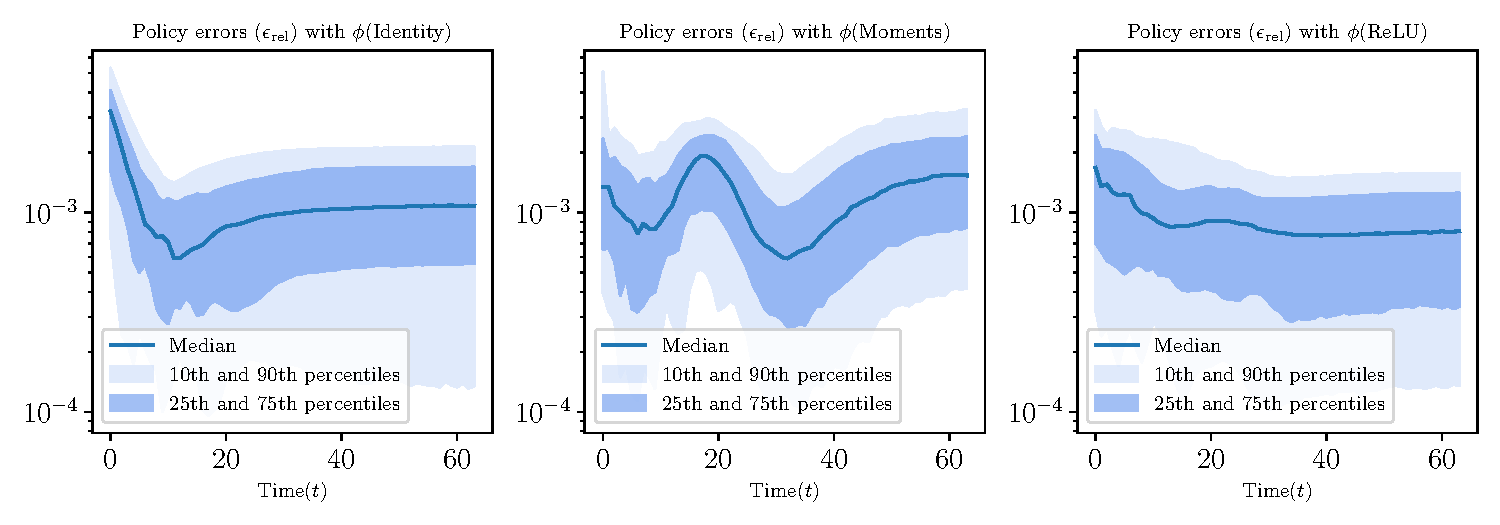
\includegraphics[height = 2.0in]{./figures/identity_moments_deep_sets_linear_relative}
			\caption{The absolute relative errors for $\nu = 1$ and $N=\mapvar{N}$ for $\phi(\text{Identity})$, $\phi(\text{Moments})$, and $\phi(\text{ReLU})$. The dark blue curve shows the median errors along equilibrium paths for \emphcolor{$\mapvar{num_seeds}$ seeds} and $\mapvar{test_trajectories}$ different trajectories.}
			\end{figure} 
		\begin{center}
				$\varepsilon \equiv \big|\frac{u(X)- \hat{u}(X)}{u(X)} \big|$
		\end{center}
		
			\end{frame}
			
			\begin{frame}{Equilibrium Paths: Linear case}
			
			\begin{figure}[h!]
			\centering
			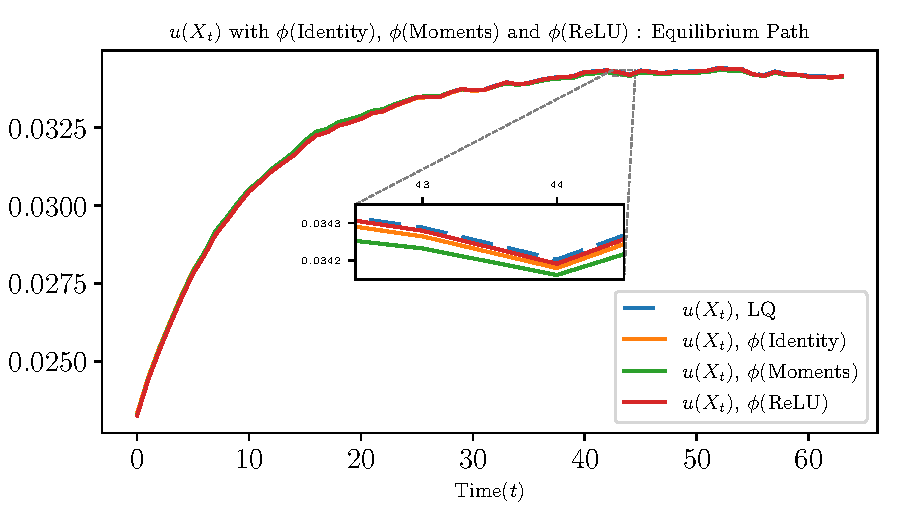
\includegraphics[height = 2.0in]{./figures/linear-baseline-theory-vs-predicted.pdf}
			\caption{Comparison between baseline approximate solutions and the LQ solution for the case with $\nu= 1$ and $N=\mapvar{N}$.}
			\end{figure}
			
			\end{frame}
			
			\begin{frame}{Computation time: Linear case}
			
			\begin{figure}[h!]
			\centering
			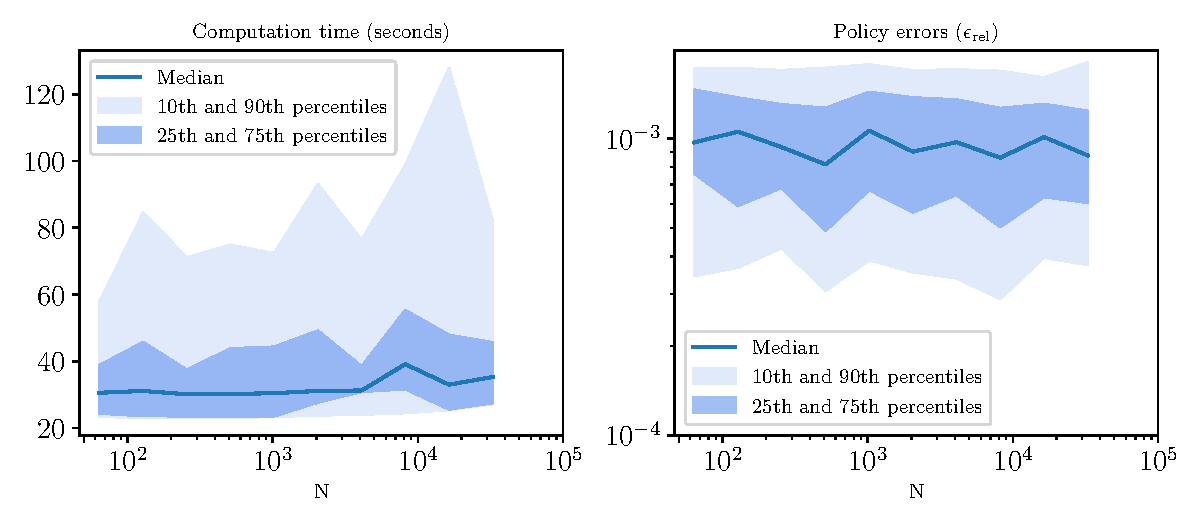
\includegraphics[height = 2.0in]{./figures/deep-sets-linear-profiling-var-n}
			\caption{Performance of the $\phi(\text{ReLU})$ for different $N$ (median value of $\mapvar{num_seeds}$ trials).}
			\end{figure}	
			
			\end{frame}
				\begin{frame}{Case 2: Nonlinear case with no ``closed-form'' solution}
				
				\begin{itemize}
				
				\item With $\nu>1$, we have a nonlinear demand function:  $p(X) = 1 -  \frac{1}{N}\sum_{i=1}^N X_i^{\nu}$.\vspace{0.1in}
				
				\item Notice how, now, the whole distribution  of $X_i$ matters.\vspace{0.1in}
				
				\item But we can still find the solution to this nonlinear case using exactly the same functional approximation and algorithm as before.\vspace{0.1in}    
				
				\item We do not need change anything in the code except the value of $\nu$.\vspace{0.1in}   
				
				\item Since the LQ solution no longer holds, we do not have an exact solution to use as a benchmark, but can check residuals.\vspace{0.1in}
				
				\item Same model and method.  Computation time by $N$ nearly the same to linear case
			
				\end{itemize}
				
				\end{frame}
	
				\begin{frame}{Euler residuals: Nonlinear case}
				
				\begin{figure}[h!]
				\centering
				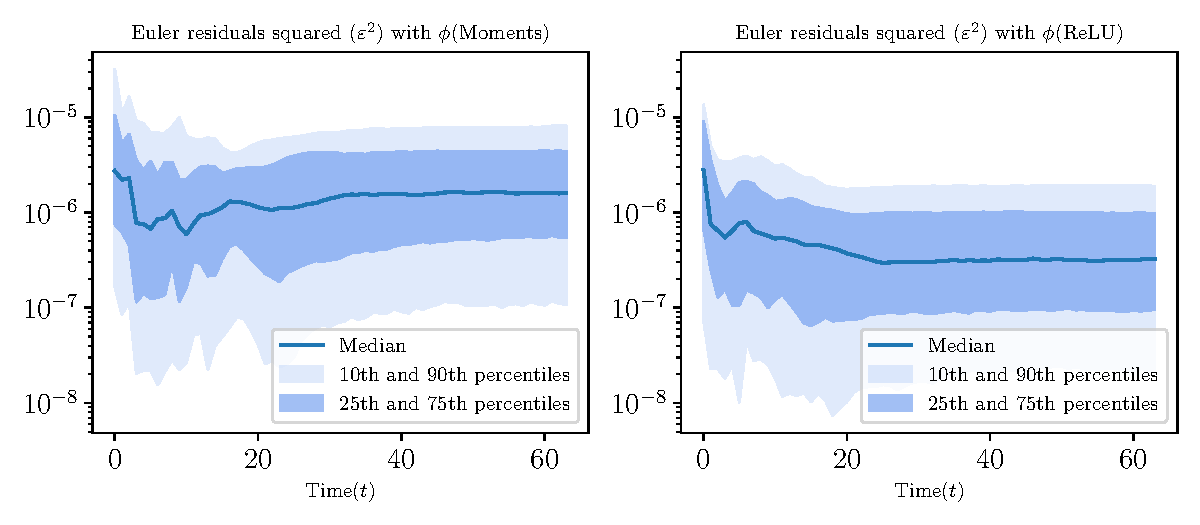
\includegraphics[height = 2.0in]{./figures/moments-deep-sets-nonlinear-residual.pdf}
				\caption{The Euler residuals for $\nu = \mapvar{nu_nonlinear_baseline}$ and $N=\mapvar{N}$ for $\phi(\text{Moments})$ and $\phi(\text{ReLU})$. The dark blue curve shows the average residuals along equilibrium paths for \emphcolor{\mapvar{num_seeds}} seeds and $\mapvar{test_trajectories}$ different trajectories.}	
				\end{figure}
				
				\end{frame}
				
				\begin{frame}{Equilibrium paths: Nonlinear case}
				
				\begin{figure}[h!]
				\centering
				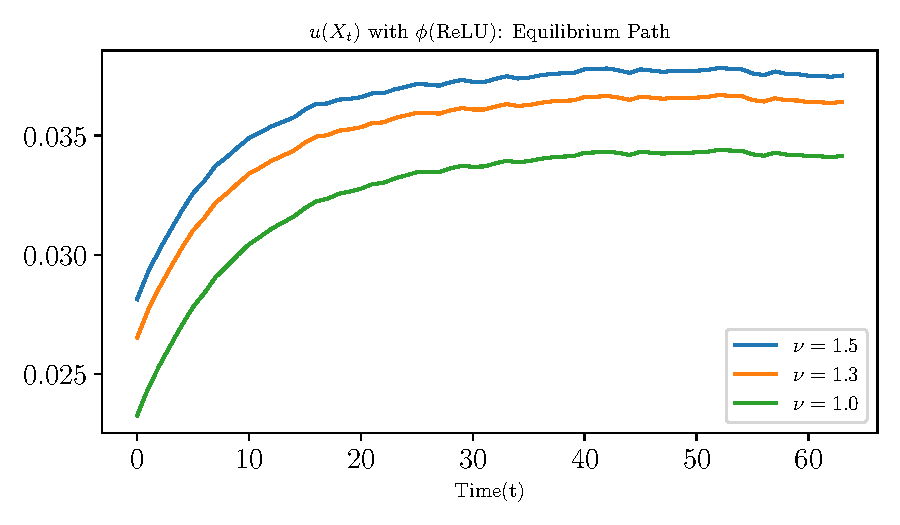
\includegraphics[width=0.7\linewidth]{./figures/deep-sets-nonlinear-var-nu.pdf}
				\caption{The optimal policy $u$ along the equilibrium paths for $\nu = [1.0,1.05,1.1,1.5]$ and $N = \mapvar{N}$. Each path shows the optimal policy for a single trajectory.}
				\end{figure}
\end{frame}



\begin{frame}{Some challenging question: Generalization puzzle}
	\emphcolor{Question I}: Generalization 
	\begin{itemize}
		\item From statistical learning and numerical analysis we know:\vspace{0.1in}
		\begin{itemize}
			\item More coefficients in the family of parametric functions $\mathcal{H}(\Theta)$ leads to over-fitting and poor generalization (bias-variance trade-off).\vspace{0.1in}
		  \item We have $\approx 200K$ parameters, and $<1K$ grid points.\vspace{0.1in}
			\item The results indicate the opposite: More coefficients $\rightarrow$ better generalization.  \vspace{0.1in}
		\end{itemize}
	\end{itemize}
How come we achieve great generalization?  
\end{frame}

\begin{frame}{Convergence results: Transversality condition and stationarity}
	\renewcommand{\arraystretch}{1.2}
	\begin{table}[h!]
		\caption{Simulating multiple seeds for different $\mathcal{H}(\Theta)$ with $\nu=1$}\vspace{-0.1in}
		\begin{center}
			\resizebox{\textwidth}{!}{\begin{tabular}{c}
					\begin{tabular}{llcccc}
\toprule
          &          & \shortstack{Success \\(\%)} & \shortstack{Early stopping failure \\ (\%)} & \shortstack{Violation of transversality\\ (\%)} & \shortstack{Overfitting \\ (\%)} \\
Group & Description &                             &                                             &                                                 &                                  \\
\midrule
Identity & Baseline &                        48\% &                                         2\% &                                            50\% &                              0\% \\
Moments & Baseline &                        59\% &                                         2\% &                                            37\% &                              2\% \\
Deep Sets & Baseline &                        97\% &                                         0\% &                                             3\% &                              0\% \\
\bottomrule
\end{tabular}

			\end{tabular}}
		\end{center}
	\end{table}
	
\end{frame}

\begin{frame}{Some challenging questions: Multiplicity and transversality puzzle}
\emphcolor{Question II}: Multiplicity and transversality 
	\begin{empheq}[box=\tcbhighmath]{align*}
		&\gamma u(X) = \beta \expec{p(X')+\gamma (1-\delta) u(X') }\\
		  X'_i & = (1-\delta)X_i + u(X) + \sigma W_i + \eta \omega,\quad\text{for } i \in \{1,...,N\}
	\end{empheq}
with linear prices. Guess and verify with $u(X) \equiv H_0 + \frac{1}{N} H_1 \sum_{i=1}^N X_i$  
\begin{itemize}
		\item The Euler equation is quadratic $\rightarrow$ \emphcolor{two} solutions: $(H_0^-, H_1^-), (H_0^+, H_1^+)$:\vspace{0.1in}
	\begin{itemize}
		\item $H_1^- <0 \rightarrow$  \emphcolor{stationary} solution, $H_1^+ > 0$ $\rightarrow$ \emphcolor{non-stationary} solution. \vspace{0.1in}
		%\item We can show $|H_1^-| < |H_1^+|$.\vspace{0.1in}
		\item We have \emphcolor{no explicit} device in our algorithm to weed out the second solution. \vspace{0.1in}
	\end{itemize}
How come there is a strong bias towards the stationary solution
	\vspace{0.1in}
	
	Understanding the \emphcolor{implicit bias} of deep neural networks answers both questions. 
\end{itemize}
\end{frame}	
				

\begin{frame}
	\frametitle{Summarizing the contribution}
	\begin{itemize}
		%\item New tools to solve (previously) \emphcolor{intractable models} (e.g. finite \# of agents)\vspace{0.1in}
		%\begin{itemize}
		%	\item Global solution starting from an initial condition.\vspace{0.1in}
		%\end{itemize}
		
		\item \emphcolor{Method} for solving \emphcolor{high-dimensional} dynamic programming problems and competitive equilibria with idiosyncratic and aggregate shocks relying\vspace{0.1in}
		\begin{itemize}
			\item Symmetry. \vspace{0.1in}
			\item Concentration of measures: Dimensionality is a \emphcolor{blessing} not a curse.\vspace{0.1in}
		\end{itemize}
		
		\item Using \emphcolor{economic theory} (i.e., exchangeability) and \emphcolor{deep learning} for function approximation with a huge \# of parameters ($\gg$ grid points)\vspace{0.1in}
		\begin{itemize}
			\item Achieve great generalization: key to alleviate the curse of dimensionality.\vspace{0.1in}
		\end{itemize}
		
		\item Implementation\vspace{0.1in}
		\begin{itemize}
			\item Can deal with $10000+$ agents.\vspace{0.1in}
			\smallskip
			\item Can deal with $10000+$ dimensional expectations with one Monte-carlo draw.\vspace{0.1in}
			\smallskip
		\end{itemize}
	\end{itemize}
\end{frame}



\section{\textcolor{PennBlue}{Spooky Boundaries at a Distance: Exploring Transversality and Stability with Deep Learning}}

\begin{frame}{Motivation}
	
	\begin{itemize}
		\item Dynamic models usually require \emphcolor{economic conditions} eliminating explosive solutions (e.g., transversality or no-bubble).\vspace{0.1in}
		\begin{itemize}
			\item These are variations of ``boundary conditions'' in ODEs and PDEs on \emphcolor{forward-looking} behavior.\vspace{0.1in}
			\item Deterministic, stochastic, sequential, recursive formulations all require conditions in some form.
			%\item Without those economic conditions, problems are not well-posed and have multiplicity
		\end{itemize}
		\medskip
		\item These forward-looking boundary conditions are the key limitation on increasing dimensionality:\vspace{0.1in}
		\begin{itemize} 
			\item Otherwise, in sequential setups, we can easily solve high-dimensional initial value problems.\vspace{0.1in}
			\item In recursive models accurate solutions are required for arbitrary values of the state variables.\vspace{0.1in}
		\end{itemize}
		\medskip
		\item \emphcolor{Question:} Can we avoid precisely calculating steady-state, BGP, and stationary distribution, which are never reached, and still have accurate short/medium-run dynamics disciplined by these boundary conditions?
	\end{itemize}
\end{frame}

\begin{frame}{Contribution}
	
	\begin{itemize}
		\item Show that \emphcolor{deep learning} solutions to many dynamic forward-looking models automatically fulfill the long-run boundary conditions we need (transversality and no-bubble).\smallskip
		\begin{itemize}
			\item We show how to design the approximation using economic insight.
		\end{itemize}
		\medskip
		\item Solve classic models with known solutions (asset pricing and neoclassical growth) and show excellent short/medium term dynamics --even when \emphcolor{non-stationary} or with \emphcolor{steady state multiplicity}.
		\medskip
		\item Suggests these methods may solve high-dimensional problems while avoiding the key computational limitation. \smallskip
		\begin{itemize}
			\item We have to understand low-dimensional problems first. 
		\end{itemize}
		\item \emphcolor{Intuition}: DL has an ``implicit bias" toward smooth and simple functions. Explosive solutions are not smooth. 
	\end{itemize}
So what is this  \emphcolor{implicit bias}?
	
\end{frame}
				
%\begin{frame}{The cure to over-fitting is to add more parameters}
%		\begin{figure}[h!]
%			\begin{center}
%				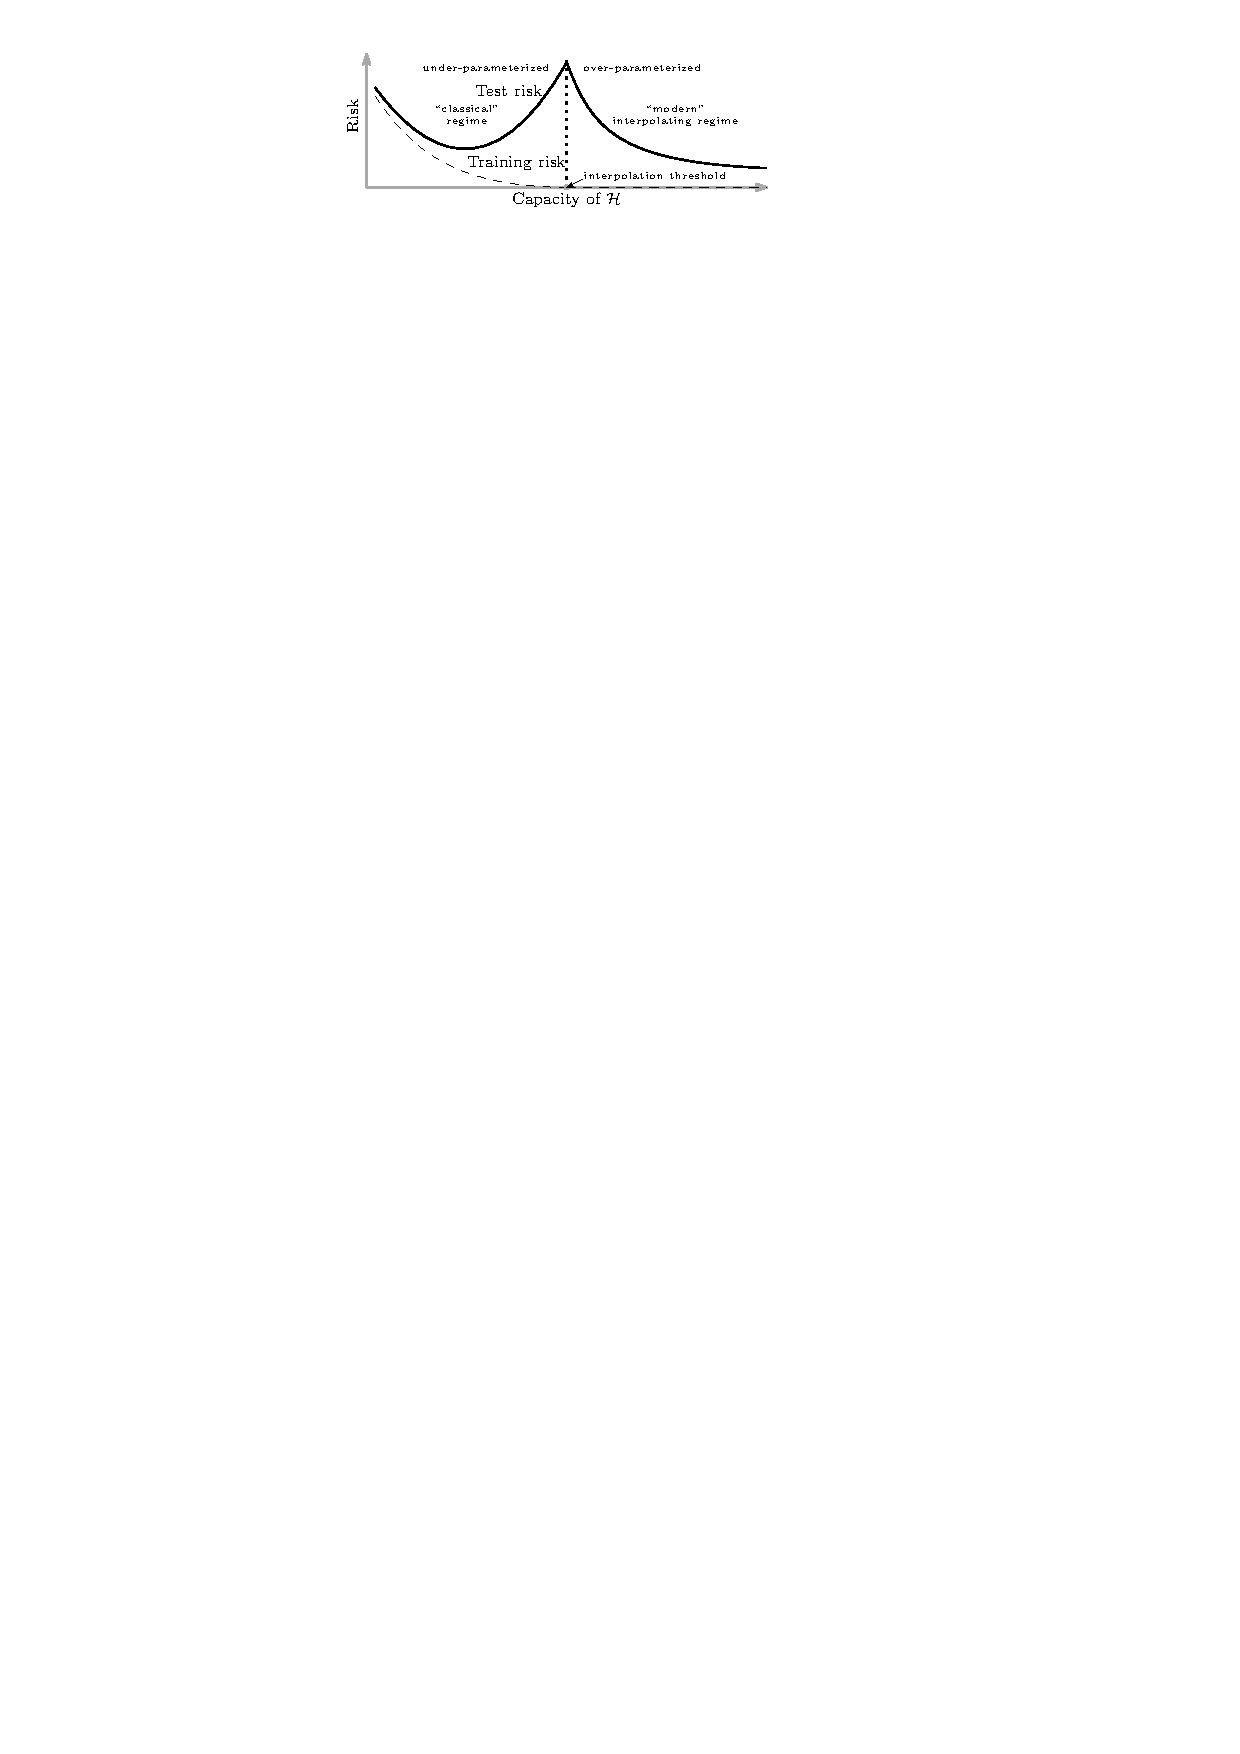
\includegraphics[height=2.0in]{./figures/doubledescent.pdf}
%			\end{center}
%		\end{figure}
%		\textcolor{red}{Belkin et al., 2019}: Traditional statistics/bias-variance trade-off stop around the interpolation threshold.		
%\end{frame}
	
\begin{frame}
	\frametitle{Deep learning optimizes in a space of functions}
		Remember 
	$$
	\min_{\theta \in \Theta} \sum_{x \in \Xtrain} \ell(\hat{\psi}(\cdot;\theta),x)^2
	$$
	\begin{itemize}
		\item Deep learning: number of coefficients is much larger than the number of grid points.\vspace{0.1in} 
		\item Since $M \gg D$, it is possible for $\hat{\psi}$ to interpolate and the objective value will be $\approx 0$.
		\vspace{0.1in}
		\item Since $M \gg D$ there are many solutions (e.g., $\theta_1$ and $\theta_2$),\vspace{0.1in}
		\begin{itemize}
			\item Agree on the grid points: $\hat{\psi}(x;\theta_1) \approx \hat{\psi}(x;\theta_2)$ for $x \in \Xtrain$.\smallskip
			%\item Agree everywhere: $\hat{f}(x;\theta_1) \approx \hat{f}(x;\theta_2)$ for $x \in \Xdom$. 
		\end{itemize}
		\medskip
		\item Since individual $\theta$ are irrelevant it is helpful to think of optimization directly within $\mathcal{H}$
		%\item Drop the $\theta$ notation to emphasize intuition of optimizing within a function space
		\begin{empheq}[box=\tcbhighmath]{equation*}
			\min_{\hat{\psi} \in \mathcal{H}} \sum_{x \in \Xtrain} \ell(\hat{\psi},x)^2\label{eq:functional-optimization}
		\end{empheq}
		\center{\Large But which $\hat{\psi}$?}
	\end{itemize}
\end{frame}

\begin{frame}
	\frametitle{Deep learning and interpolation}\label{implicit}
	\begin{itemize}
		\item For $M$ large enough, optimizers \emphcolor{tend to} converge to \emphcolor{unique} \emphcolor{``simple"}  $\hat{\psi}$ (w.r.t to some norm $\|\cdot\|_S$). Unique both in $\Xtrain$ and $\Xdom$. There is a \emphcolor{bias} toward a specific class of solutions.
		\medskip
		\item \emphcolor{How to interpret:} interpolating solutions for some functional norm $\|\cdot\|_S$
		\begin{empheq}[box=\tcbhighmath]{align*}
			\min_{\hat{\psi}\in \mathcal{H}} &||\hat{\psi}||_S\\
			\st & \ell(\hat{\psi},x)=0,\quad \text{ for } x \in \Xtrain
		\end{empheq}
		\vspace{-0.1in}
		
		\begin{itemize}
			\item Comp Sci literature refers to this as the \emphcolor{inductive bias} or \emphcolor{implicit bias}: optimization process is biased toward particular $\hat{\psi}$.\smallskip
			\item Small values of $\|\cdot\|_S$ corresponds to \emphcolor{flat} solutions with \emphcolor{small gradients} (w.r.t. input).
			\smallskip
			\item Characterizing $\|\cdot\|_S$  is an active research area in CS at the heart of deep learning theory.
		\end{itemize}
	\end{itemize}
\hyperlink{sobolev}{\beamerskipbutton{Sobolev}}
\end{frame}


\begin{frame}{Flat and smooth interpolation:  Illustration}
	\begin{figure}[h!]
		\begin{center}
			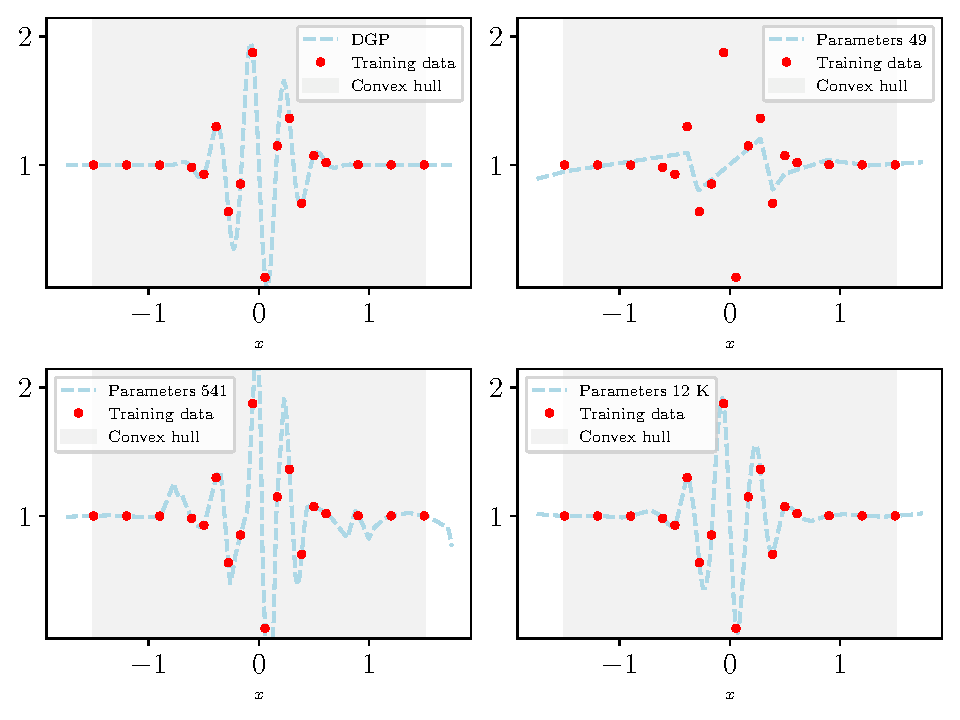
\includegraphics[height=2.7in]{./figures/fourplots_example_reg.pdf}
		\end{center}
	\end{figure}

\end{frame}

\begin{frame}
	\frametitle{Deep learning and interpolation in practice}
	\emphcolor{Reminder}: in practice we solve
	\begin{empheq}[box=\tcbhighmath]{equation*}
		\min_{\theta \in \Theta} \sum_{x \in \Xtrain} \ell\left(\hat{\psi}(\cdot;\theta),x\right)^2
	\end{empheq}
	\begin{itemize}
		\item The smooth interpolation is imposed \emphcolor{implicitly} through the optimization process.
		\item No explicit norm minimization or penalization is required.
		%\item  The optimization methods designed for over-parameterized approximation \emphcolor{implicitly} provides it.
	\end{itemize}
	\emphcolor{In this paper:} we describe how (and when) the $\min_{\hat{\psi}\in \mathcal{H}} ||\hat{\psi}||_S$ solutions are also the ones which  automatically fulfill transversality and no-bubble conditions.  
	\begin{itemize}
		\item They are disciplined by long-run boundary conditions. Therefore, we can obtain accurate short/medium-run dynamics. 
	\end{itemize}
\end{frame}

\begin{frame}{Outline}
	
	To explore how we can have accurate short-run dynamics, we show deep learning solutions to
	\begin{enumerate}
		\item Classic linear-asset pricing model.\vspace{0.1in}
		\item Sequential formulation of the neoclassical growth model.\vspace{0.1in}
		\item Sequential neoclassical growth model with multiple steady states.\vspace{0.1in}
		\item Recursive formulation of the neoclassical growth model.\vspace{0.1in}
		\item  Non-stationarity, such as balanced growth path.\vspace{0.1in}
		
	\end{enumerate}
	
\end{frame}

\section{Linear asset pricing}

\begin{frame}{Sequential formulation}
	\begin{itemize}
		\item Dividends, $y(t)$, $y_0$ as given, and follows the process:
		\begin{equation*}
			y(t+1) = c + (1+g) y(t)
		\end{equation*}
		\item Writing as a linear state-space model with $x(t+1) = A x(t)$ and $y(t) = G x(t)$ and
		\begin{align*}
			x(t) \equiv \begin{bmatrix*}
				1 & y(t)
			\end{bmatrix*}^\top, A \equiv \begin{bmatrix*}
				1 & 0   \\
				c & 1+g
			\end{bmatrix*}, G \equiv \begin{bmatrix*}
				0 & 1
			\end{bmatrix*}
		\end{align*}
		\item ``Fundamental'' price given $x(t)$ is PDV with $\beta \in (0,1)$ and $\beta(1+g) < 1$
		\begin{empheq}[box=\tcbhighmath]{equation*}
			p_f(t) \equiv \sum_{j=0}^\infty \beta^j y({t+j}) = G(I - \beta A)^{-1} x(t).
		\end{empheq}
	\end{itemize}
\end{frame}

\begin{frame}{Recursive formulation}
	With standard transformation, all solutions $p_f(t)$ fulfill the recursive equations
	\begin{align}
		\quad & p(t)  = G x(t) + \beta p(t+1)\label{eq:recursive-p-t}                            \\
		\quad & x(t+1)  = A x(t) \label{eq:lom-x}                                               \\
		\quad & 0    = \lim_{T \rightarrow \infty} \beta^T p(T) \label{eq:no-bubble-condition-T} \\
		\quad & x_0      \text{ given}\vspace{0.1in}\label{eq:initial-x0}
	\end{align}
	That is, a system of two difference equations with one boundary and one initial condition.
	\begin{itemize}
		\item The boundary condition \cref{eq:no-bubble-condition-T} is an \emphcolor{condition} necessary for the problem to be well-posed and have a unique solution.
		\item It ensures that $p(t) = p_f(t)$ by imposing long-run boundary condition.
		\item But without this assumption there can be ``bubbles'' with $p(t) \neq p_f(t)$, only fulfilling \cref{eq:recursive-p-t,eq:lom-x}.
		\item Intuition: system of $\{p(t), x(t)\}$ difference equations requires total of two boundaries or initial values to have a unique solution.
	\end{itemize}
	
\end{frame}


\begin{frame}{Solutions without no-bubble condition}
	Without the no-bubble condition:
	\begin{itemize}
		\item Solutions in this deterministic asset pricing model are of the form:
		\begin{empheq}[box=\tcbhighmath]{equation}
			p(t) = p_f(t)+\zeta~ \beta^{-t}. \label{eq:sol-seq-with-bubble}
		\end{empheq}
		\item For any $\zeta \geq 0$.  The initial condition $x(0)$ determines  $p_f(t)$.
		\item There are infinitely many solutions.  
		\item The no-bubble condition chooses  $\zeta = 0$.
	\end{itemize}
	
	%Lets analyze this with a ``deep learning'' solution, first by imposing the no-bubble condition.
	
\end{frame}

\begin{frame}{Interpolation problem: without no-bubble condition}
	\begin{itemize}
		\item A set of points in time $\Xtrain = \{t_1,\ldots,t_{\text{max}}\}$.
		\item A family of over-parameterized functions $p(\cdot;\theta) \in \mathcal{H}(\Theta)$.
		\item Generate $x(t)$ using the law of motion and $x(0)$, equation \cref{eq:lom-x}.
		
		In practice we minimize the residuals of the recursive form for the price:
		\begin{empheq}[box=\tcbhighmath]{align}
			\min_{\theta \in \Theta} \frac{1}{|\Xtrain|}\sum_{t \in \Xtrain} \left[p(t;\theta)- G x(t)- \beta p(t+1;\theta)\right]^2
		\end{empheq}
		\item This minimization \emphcolor{does not contain}  no-bubble condition. It has infinitely many minima.
		\item Does the implicit bias of over-parameterized interpolation weed out the bubbles? \emphcolor{Yes}.
		\item  \emphcolor{Intuition}: bubble solutions are explosive, i.e., big functions with big derivatives.
		\bigskip
		
		Let's analyze this more rigorously. 
	\end{itemize}
\end{frame}

\begin{frame}{Interpolation formulation: min-norm mental model}
	The min-norm \emphcolor{interpretation} (mental model) is:
	\begin{empheq}[box=\tcbhighmath]{align}
		\min_{p \in \mathcal{H}} \quad & \|p\|_S\\
		\st \quad & p(t)- G x(t)- \beta p(t+1) = 0 \quad \text{for } t  \in \Xtrain \label{eq:p-t-deep} \\
		\quad & 0 = \lim_{T \rightarrow \infty} \beta^T p(T) \label{eq:no-bubble-condition-deep}
	\end{empheq}
	Where $x(t)$ for $t  \in \Xtrain$ is defined by $x(0)$ initial condition and recurrence $x(t+1) = A x(t)$ in \cref{eq:lom-x}
	\begin{itemize}
		%\item Recall: generalization comes from design of $\mathcal{H}$ and optimizer; not only model, i.e., \cref{eq:p-t-deep,eq:no-bubble-condition-deep}.\medskip
		\item The minimization of norm $\|p\|_S$ is the ``inductive bias'' toward particular solutions for $t \in [0,\infty] \setminus \Xtrain$.\medskip
		%\item What types of norms $\|p\|_S$ would $\mathcal{H}$ and optimization induce? CS theory suggests variations Sobolev.
	\end{itemize}
\end{frame}

\begin{frame}{Is the no-bubble condition still necessary?}
	
	\begin{itemize}
		\item To analyze, drop the no-bubble condition and examine the class of solutions. 
		\item In this case, we know the interpolating solutions to \cref{eq:p-t-deep} without imposing \cref{eq:no-bubble-condition-deep}
		\begin{equation}
			p(t) = p_f(t) + \zeta \beta^{-t}%= G (I-\beta A)^{-1}x_t + \zeta \beta^{-t}
		\end{equation}
		\item Applying the triangle inequality
		\begin{empheq}[box=\tcbhighmath]{align}
			\|p_f\|_S \leq \|p\|_S \leq \|p_f\|_S + \zeta~ \|\beta^{-t}\|_S\label{eq:asset-pricing-triangle}
		\end{empheq}
		\item Relative to classic methods the ``deep learning'' problem now has a new objective, minimizing $\|p\|_S$.\smallskip
		\medskip
		\item The new objective of minimizing the norm, makes the no-bubble condition \emphcolor{redundant}.
	\end{itemize}
\end{frame}

\begin{frame}[label = asset_seq]{Min-norm norm formulation: redundancy of no-bubble condition}
	
	Given the no-bubble condition is automatically fulfilled, could solve the following given some $\mathcal{H}$ and compare to $p_f(t)$
	\begin{empheq}[box=\tcbhighmath]{align}
		\min_{p \in \mathcal{H}} \quad & \|p\|_S\\
		\st \quad & p(t)- G x(t)- \beta p(t+1) = 0 \quad \text{for } t  \in \Xtrain
	\end{empheq}
	A reminder: in practice, given the $\Xtrain$, we directly implement this as $p(\cdot;\theta) \in \mathcal{H}(\Theta)$ and fit with
	\begin{empheq}[box=\tcbhighmath]{align}
		\min_{\theta \in \Theta} \frac{1}{|\Xtrain|}\sum_{t \in \Xtrain} \left[p(t;\theta)- G x(t)- \beta p(t+1;\theta)\right]^2
	\end{empheq}
	Since law of motion is deterministic, given $x(0)$ we generate $x(t)$ with $x(t+1) = A x(t)$ for $t  \in \Xtrain$
	\begin{itemize}
		\item The $\Xtrain$ does not need to be contiguous and $|\Xtrain|$ may be relatively small.
		\item Most important: no steady state calculated, nor large $T \in \Xtrain$ required.
	\end{itemize}
\end{frame}

\begin{frame}
	\frametitle{Results}
	\begin{figure}[htb]
		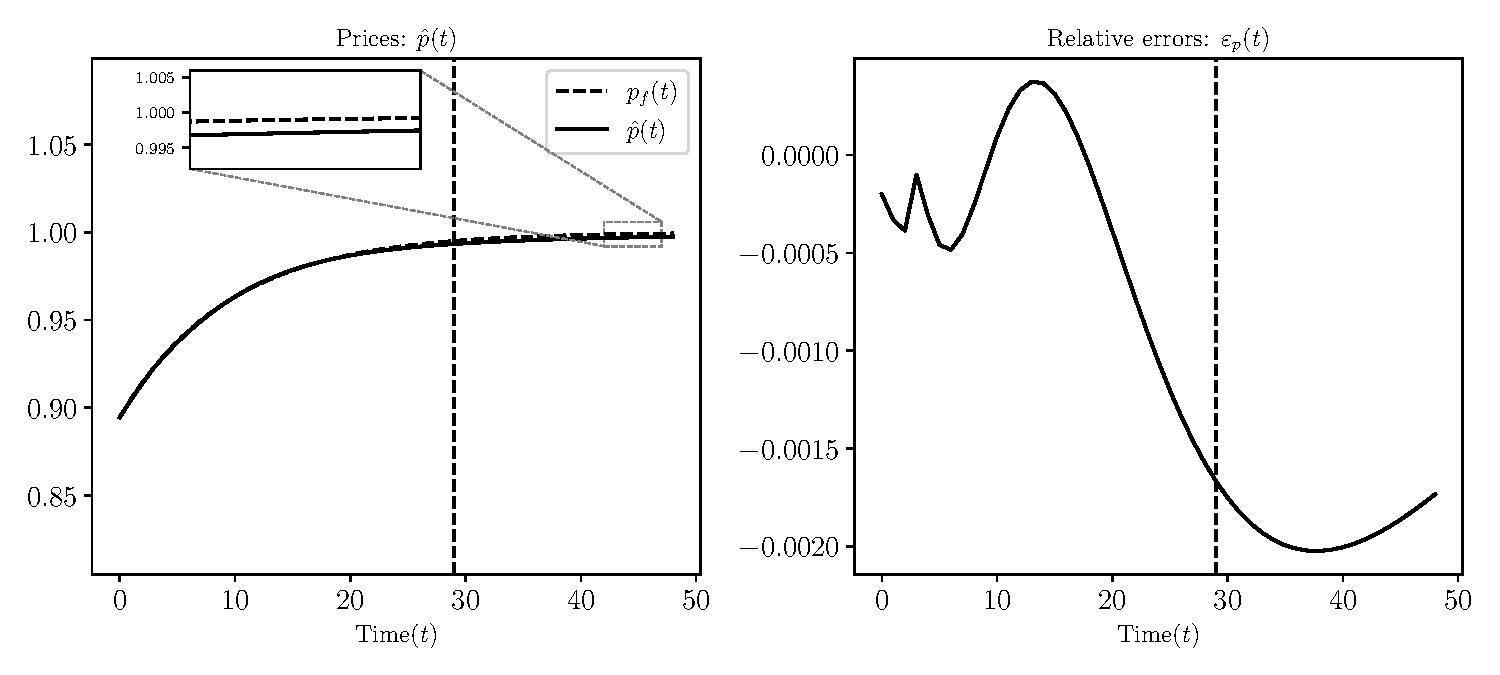
\includegraphics[width=10cm]{./figures/asset_seq_g0.pdf}
	\end{figure}
	\begin{enumerate}
		%\item Relative Error: $\frac{p(t)-p^f(t)}{p^f(t)}$.  Extrapolation is $t > 30 = \max_t \Xtrain$
		\item \emphcolor{Pick} $\Xtrain =\{0,1,2,...,29\}$ and $t > 29$ is ``extrapolation'' where $c=0.01$, $g = -0.1$, and $y_0 = 0.8$.
		\item \emphcolor{Choose} $p(t;\theta) = NN(t;\theta)$ where ``NN'' has $4$ hidden layers of $128$ nodes. $|\Theta| = 49.9 K$ coefficients.
		\item \emphcolor{Fit} using L-BFGS and PyTorch in just a \emphcolor{few seconds}. Could use Adam/SGD/etc.
		\item Low generalization errors, even without imposing no-bubble condition.
		%\begin{itemize}
		%   \item Relative error $\equiv  \frac{p(t)-p^f(t)}{p^f(t)}$ ranging from $0.07\%$ for $t=0$ to $0.25 \%$ when extrapolating.
		%  \item These long run errors don't affect the short-run accuracy (still small, even after we are all dead)
		%\end{itemize}
	\end{enumerate}
	\begin{center}
			$\varepsilon_p(t)\equiv \frac{\hat{p}(t)-p(t)}{p(t)}$.
	\end{center}
\end{frame}

\begin{frame}{Contiguous vs. sparse grid}
	\begin{minipage}[t]{0.4\textwidth}
		\raisebox{-\height+0.7\baselineskip}{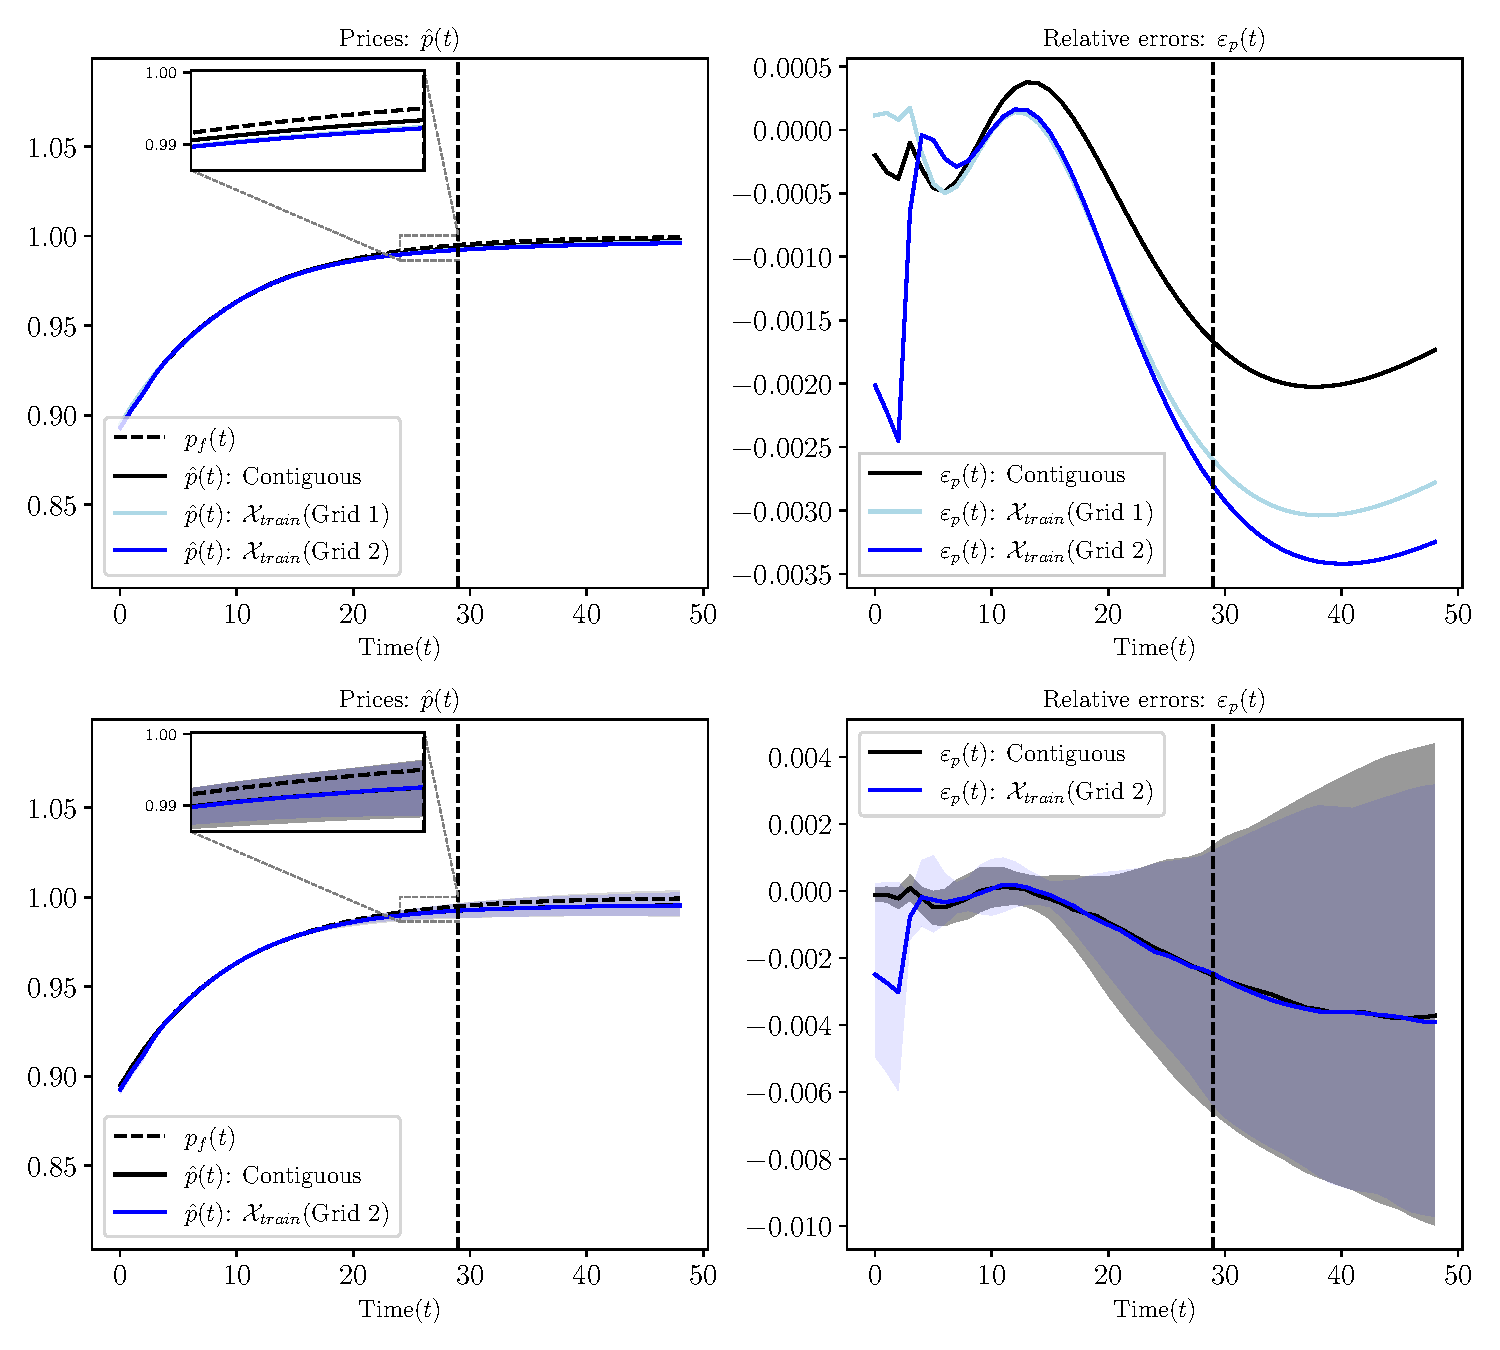
\includegraphics[width= 8cm]{./figures/asset_pricing_seq_g0_grids.pdf}}
		%\includegraphics[width=8cm]
	\end{minipage}
	\hfill%
	\begin{minipage}[t]{0.5\textwidth}\raggedleft
		\begin{itemize}
			\item \emphcolor{Pick} $\Xtrain({\text{Grid 1}})  = \{0, 1, 2, 4, 6, 8, 12, 16, 20, 24, 29\}$ and $\Xtrain({\text{Grid 2}}) = \{0, 1, 4, 8, 12, 18, 24, 29\}$.
			\smallskip
			\item Contrary to popular belief, can use \emphcolor{less grid points} relative to alternatives. 
			%\item The same neural network with $|\Theta| = 49.9 K$.
			%\item Shaded regions: $10$th and $90$th percentiles over $100$ seeds:
			\smallskip
				\item Hypothesis verified, the solutions agree on the seen and \emphcolor{unseen} grid points. \smallskip
		\end{itemize}
	\end{minipage}
\end{frame}


\section{Neoclassical growth in sequence space}

\begin{frame}{Sequential formulation}
	\begin{align}
		\max_{\{c(t),k(t+1)\}_{t=0}^\infty} \quad & \sum_{t=0}^\infty \beta^t u\left(c(t)\right) \\
		\st\quad & k(t+1) = z(t)^{1-\alpha}f\left(k(t)\right) + (1-\delta)k(t) - c(t) \\
		\quad & z(t+1)=(1+g)z(t)\label{eq:lom-z-sequential}\\
		& k(t)\geq 0 \\
		\quad & 0 = \lim_{T\rightarrow \infty} \beta^T u'\left(c(T)\right)k(T+1)\label{eq:transversality-rbc-sequential} \\
		& k_0,z_0  \text{ given }
	\end{align}
	
	\begin{itemize}
		\item Preferences: $u(c) = \frac{c^{1-\sigma}-1}{1-\sigma}$, $\sigma > 0$, $\lim_{c\rightarrow 0} u'(c) = \infty$, and $\beta \in (0,1)$.
		\item Cobb-Douglas production function: $f(k) = k^{\alpha}$, $\alpha \in (0,1)$ before scaling by TFP $z_t$.
		\item Skip standard steps\ldots Euler equation: $u'(c(t)) = \beta u'(c(t+1)) \big[z(t+1)^{1-\alpha} f'(k(t+1)) + 1-\delta\big]$.
	\end{itemize}
\end{frame}


\begin{frame}{Interpolation problem: without transversality condition}
	\begin{itemize}
		\item A set of points in time $\Xtrain = \{t_1,\ldots,t_{\text{max}}\}$.
		\item A family of over-parameterized functions $k(\cdot;\theta) \in \mathcal{H}(\Theta)$.
		\item Generate $z(t)$ using the law of motion and $z(0)$, equations \cref{eq:lom-z-sequential}.
		\item Use the feasibility condition and define $c(t;k)\equiv z(t)^{1-\alpha}f\big(k(t)\big) + (1-\delta)k(t)-k(t+1)$.\vspace{5mm}
		
		In practice we minimize the Euler and initial conditions residuals:
		\begin{empheq}[box=\tcbhighmath]{align*}
			\min_{\theta \in \Theta}  \bigg(\frac{1}{|\Xtrain|}\sum_{t \in \Xtrain} & \lambda_1 \bigg[ \underbrace{ \frac{u'\big(c(t;k(\cdot,\theta))\big)}{u'\big(c(t+1;k(\cdot;\theta))\big)} -\beta\big[z(t+1)^{1-\alpha} f'(k(t+1;\theta)) + 1-\delta\big] }_{\text{Euler residuals}}\bigg]^2 \\  + \lambda_2
			&  \bigg[\underbrace{k(0;\theta)-k_0}_{\text{Initial condition residuals}}\bigg]^2\bigg)
		\end{empheq}
		\item $\lambda_1$ and $\lambda_2$ positive weights.
	\end{itemize}
\end{frame}

\begin{frame}{Interpolation problem: without transversality condition}
	\begin{itemize}
		\item This minimization \emphcolor{does not contain } the transversality condition.			\smallskip
		\begin{itemize}
			\item Without the transversality condition it has infinitely many minima.
		\end{itemize}
		\bigskip
		\item \emphcolor{No explicit} norm minimization.
		\bigskip	
		\item Does the implicit bias  weed out the solutions that violate the transversality condition? \emphcolor{Yes}. 
		\bigskip 
		\item \emphcolor{Intuition}: The solutions that violate the transversality condition are big functions with big derivatives.
		\bigskip
		
		Let's analyze this more rigorously.
	\end{itemize}
\end{frame}

\begin{frame}{Interpolation formulation: min-norm mental model}
	\begin{empheq}[box=\tcbhighmath]{align}
		\min_{k \in \mathcal{H}} \quad & \|k\|_S\\
		\st \quad & u'(c(t;k)) = \beta u'(c(t+1;k)) \big[z(t+1)^{1-\alpha} f'(k(t+1)) + 1-\delta\big] \quad \text{for } t \in \Xtrain\label{eq:seqgrowtheuler} \\
		\quad & k(0) = k_0 \label{eq:rbc-initial-condition}\\
		\quad & 0 = \lim_{T\to\infty}\beta^T u'(c(T;k))k(T+1) \label{eq:rbc-transversality}
	\end{empheq}
	\begin{empheq}[box=\tcbhighmath]{align}
		c(t;k) \equiv z(t)^{1-\alpha}f\big(k(t)\big) + (1-\delta)k(t)-k(t+1) \label{eq:seqgrowthlom}
	\end{empheq}
	Where $z(t)$ for $t  \in \Xtrain$ is defined by $z(0)$ initial condition and recurrence $z(t+1) = (1+g) z(t)$.
\end{frame}


\begin{frame}[label = NCG_Minnorm]{Is the transversality condition still necessary? Case of g = 0, z = 1 }
	
	Sketch of the proof:
	\begin{itemize}
		\item Let $\{k(t),c(t)\}$ be the sequence of optimal solution.
		\item Let $\{\tilde{k}(t),\tilde{c}(t)\}$ be a sequence of solution that satisfy all the equations \emphcolor{except} transversality condition \cref{eq:rbc-transversality}.
	\end{itemize}
	
	\begin{enumerate}
		\item $\tilde{c}(t)$ approaches zero.
		\item $\tilde{k}(t)$ approaches $\tilde{k}_{\text{max}}\equiv\delta^{\frac{1}{\alpha-1}}$, and $k(t)$ approaches $k^*\equiv \left(\frac{\beta^{-1}+\delta-1}{\alpha}\right)^{\frac{1}{\alpha-1}}$. 
		\item Both $\tilde{k}(t)$ and $k(t)$ are monotone. $\tilde{k}_{\text{max}} \gg k^*$. Therefore,
		\begin{align*}
			0 \leq \|k\|_S \leq \|\tilde{k}\|_S.
		\end{align*}
	\end{enumerate}
	
	
\end{frame}

\begin{frame}[label =TVC_Examples]{Is the transversality condition still necessary? Case of g = 0, z = 1 }
	
	Example: the violation of the transversality condition.
	\begin{figure}[htb]
		\centering
		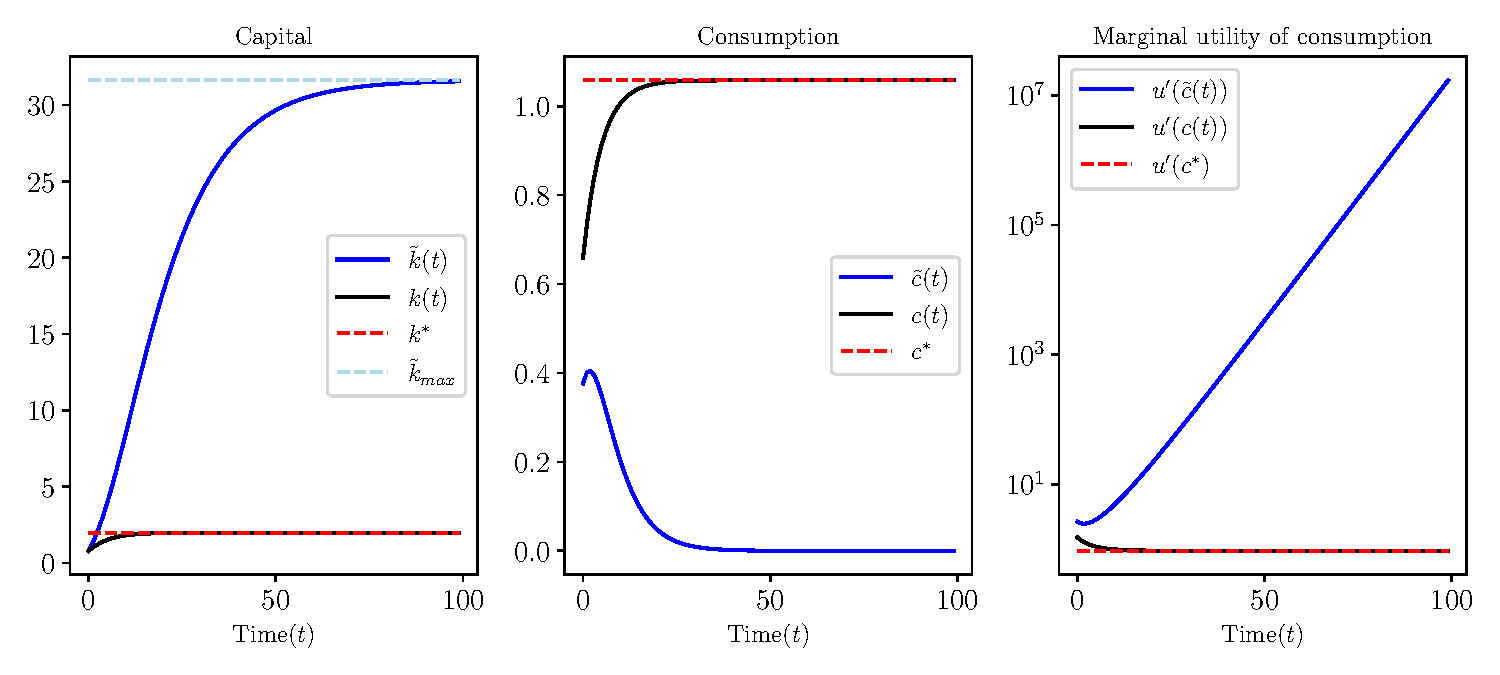
\includegraphics[width=11cm]{./figures/growth_sequential_violating_tvc_paths_below.pdf}
	\end{figure}
	
	\begin{itemize}
		\item The solution that violate the transversality are associated with \emphcolor{``big"} capital path.
		\item The new objective of minimizing the norm, makes the transversality condition \emphcolor{redundant}.
	\end{itemize}
	

\end{frame}

\begin{frame}[label = ncg_seq]{Min-norm formulation: redundancy of transversality condition}
	Given the transversality condition is automatically fulfilled, one could solve 
	\begin{empheq}[box=\tcbhighmath]{align*}
		\min_{k \in \mathcal{H}} \quad & \|k\|_S\\
		\st \quad & u'(c(t;k)) = \beta u'(c(t+1;k)) \big[z(t+1)^{1-\alpha} f'(k(t+1)) + 1-\delta\big] \quad \text{for } t \in \Xtrain \\
		\quad & k(0) = k_0
	\end{empheq}
	Reminder: in practice we solve
	\begin{align*}
		\min_{\theta \in \Theta}  \bigg(\frac{1}{|\Xtrain|}\sum_{t \in \Xtrain} & \lambda_1 \bigg[ \frac{u'\big(c(t;k(\cdot,\theta))\big)}{u'\big(c(t+1;k(\cdot;\theta))\big)} -\beta\big[z(t+1)^{1-\alpha} f'(k(t+1;\theta)) + 1-\delta\big]\bigg]^2 \\  + \lambda_2
		&  \bigg[\underbrace{k(0;\theta)-k_0}_{\text{Initial condition residuals}}\bigg]^2\bigg)
	\end{align*}
	\begin{itemize}
		\item $|\Xtrain|$ may be relatively small,  no steady state calculated, nor large $T \in \Xtrain$ required.
	\end{itemize}
\end{frame}

\begin{frame}[label = res_seq_ncg]{Results}
	
	\begin{figure}[htb]
		\centering
		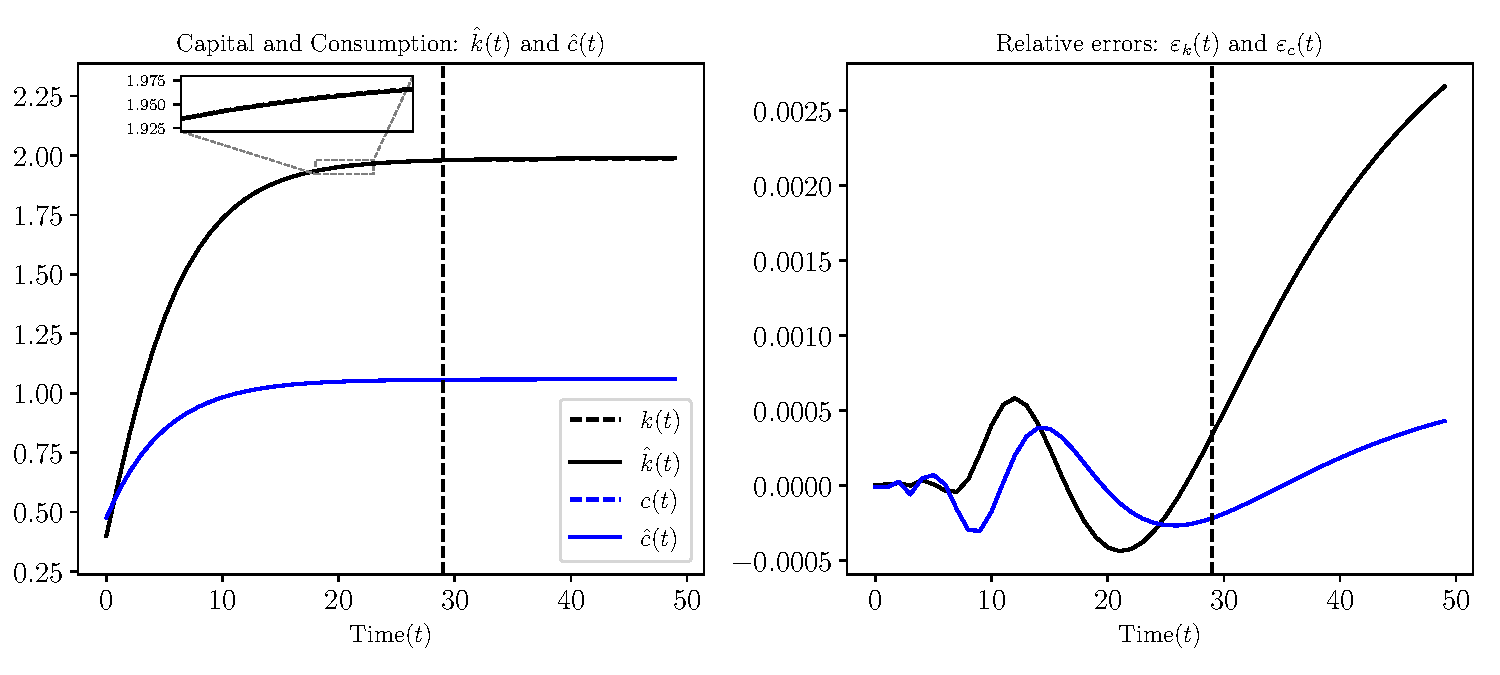
\includegraphics[width=10cm]{./figures/growth_seq_g0_one_run.pdf}
	\end{figure}
	
	\begin{enumerate}
		%\item Relative Error: $\frac{p(t)-p^f(t)}{p^f(t)}$.  Extrapolation is $t > 30 = \max_t \Xtrain$
		\item \emphcolor{Pick} $\Xtrain =\{0,1,...,30\}$ and $t > 30$ is ``extrapolation''  $\alpha=\frac{1}{3}$, $\sigma =1$, $\beta = 0.9$, $g = 0.0$, and $k_0 = 0.4$
		\item \emphcolor{Choose} $k(t;\theta) = NN(t;\theta)$ where ``NN'' has $4$ hidden layers of $128$ nodes. $|\Theta| = 49.9 K$ coefficients.
		\item \emphcolor{Fit} using L-BFGS in just a \emphcolor{few seconds}. Comparing with value function iteration solution.
		\item Low generalization errors, even without imposing the transversality condition. 
	\end{enumerate}
	Relative errors defined as $\varepsilon_c(t)\equiv \frac{\hat{c}(t)-c(t)}{c(t)}$, $\varepsilon_k(t)\equiv \frac{\hat{k}(t)-k(t)}{k(t)}$.
\end{frame}

\begin{frame}[label = TFP_seq_ncg]{Growing TFP}
	\begin{minipage}[t]{0.4\textwidth}
		\raisebox{-\height+0.7\baselineskip}{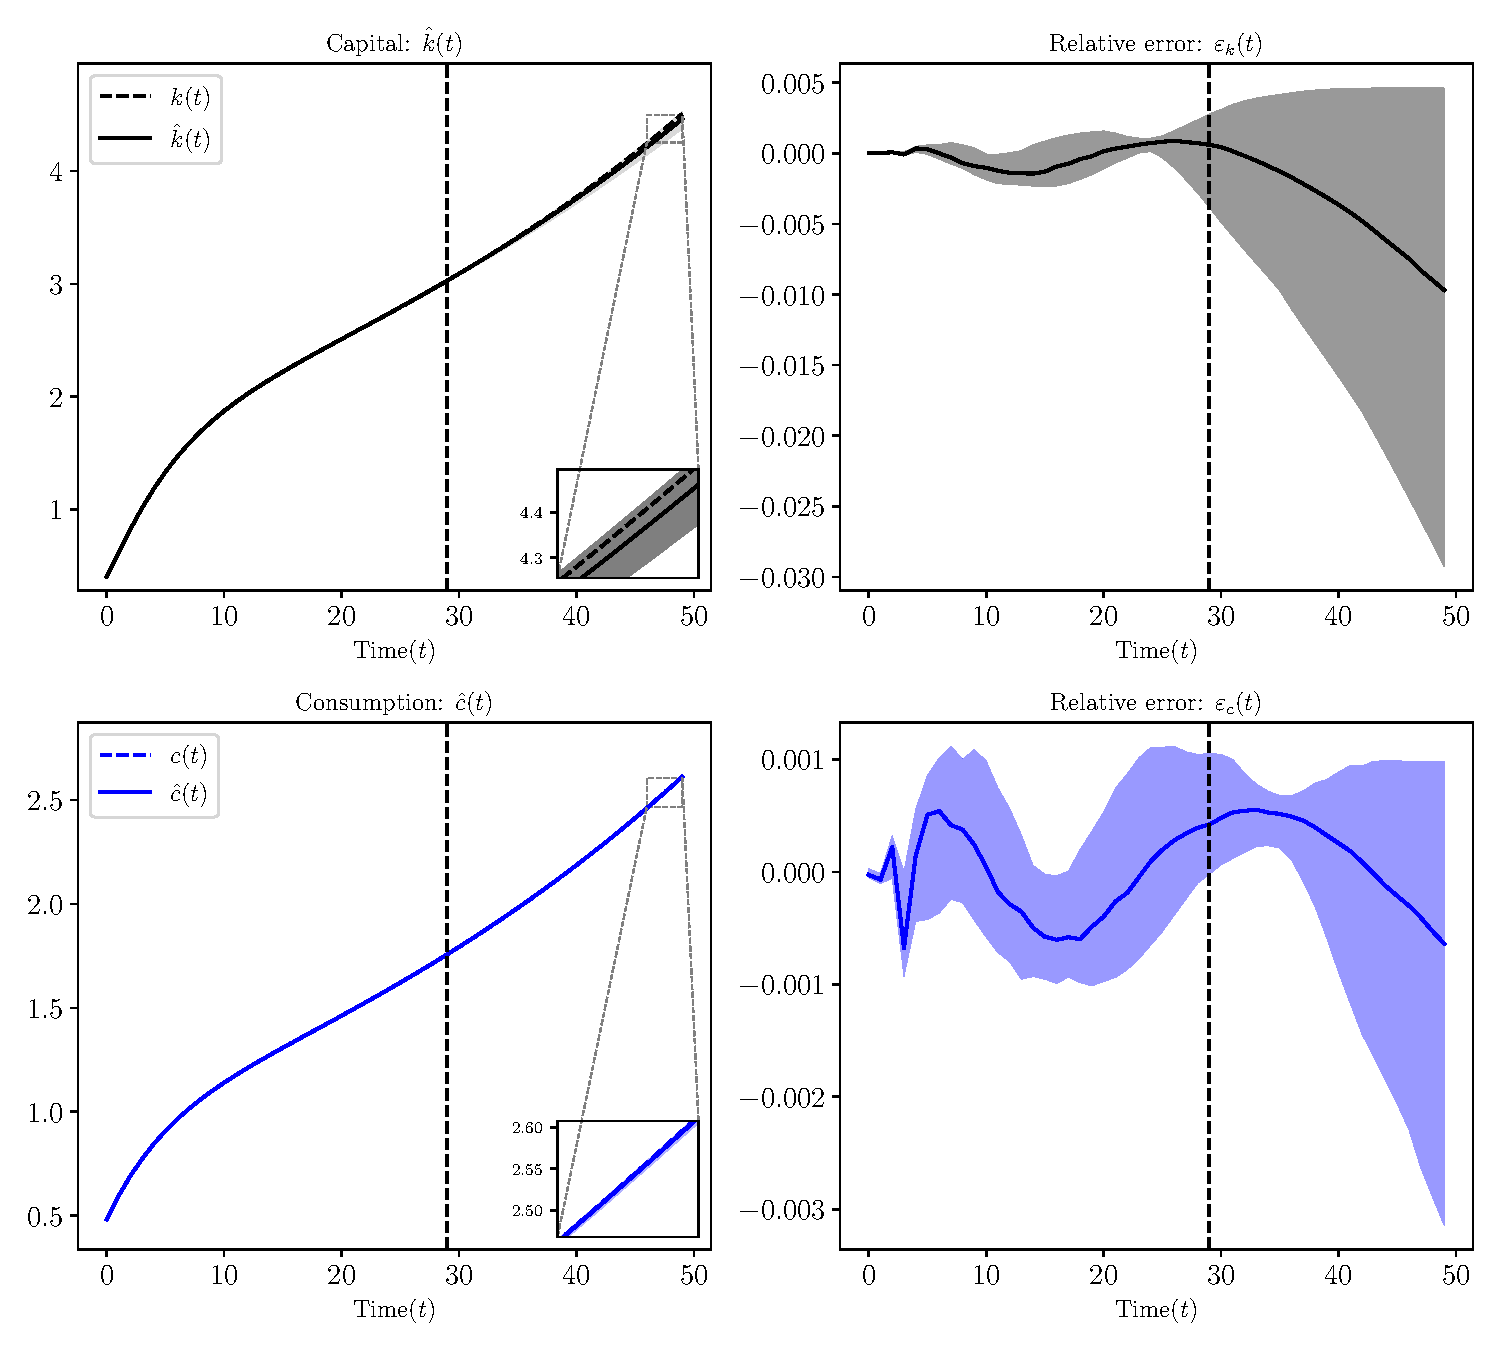
\includegraphics[width= 8cm]{./figures/growth_seq_g_positive_ensemble.pdf}}
		%\includegraphics[width=8cm]
	\end{minipage}
	\hfill%
	\begin{minipage}[t]{0.5\textwidth}\raggedleft
		\begin{itemize}
			\item \emphcolor{Pick} same $\Xtrain$ but now $g = 0.02$.
			\item \emphcolor{Choose} $k(t;\theta) = e^{\phi t} NN(t;\theta_{NN})$ where $\theta \equiv \{\phi,\theta_{NN}\}\in\Theta$ is the coefficient vector
			\begin{itemize}
				\item Here we used economic intuition of problem to design the $\mathcal{H}(\Theta)$ to generalize better.
			\end{itemize}
			\item Non-stationary but can figure out the BGP.
			\item  Learns the growth rate: $\phi \approx \ln(1+g)$ 
			\item Economic insight leads to great extrapolation!
		\end{itemize}
	\end{minipage} 
\end{frame}

\section{The neoclassical growth model with multiple steady states}
\begin{frame}{Sequential formulation}
	
	\begin{align*}
		\max_{\{c_t,k_{t+1}\}_{t=0}^\infty} \quad & \sum_{t=0}^\infty \beta^t u(c_t)                      \\
		\st\quad                                  & k_{t+1} = f(k_t) + (1-\delta)k_t - c_t                \\
		& k_{t}\geq0                                            \\
		\quad                                     & 0 = \lim_{T\rightarrow \infty} \beta^T u'(c_T)k_{T+1} \\
		& k_0  \text{ given.}
	\end{align*}
	\begin{enumerate}
		\item Preferences: $u(c) = \frac{c^{1-\sigma}-1}{1-\sigma}$, $\sigma > 0$, $\lim_{c\rightarrow 0} u'(c) = \infty$, and $\beta \in (0,1)$.			\smallskip
		\item \emphcolor{``Butterfly production function"}: $f(k) = a \max\{k^\alpha, b_1 k^\alpha - b_2\}$, $\alpha \in (0,1)$:
		\smallskip
		\begin{itemize}
			
			\item There is a kink in the production function at $k^* \equiv \big(\frac{b_2}{b_1 -1}\big)^\frac{1}{\alpha} $.			\smallskip
			
			\item This problem has \emphcolor{two} steady states, $k_1^*$ and $k_2^*$ and their corresponding consumption levels $c_1^*$ and $c_2^*$.
		\end{itemize}
	\end{enumerate}
\end{frame}

\begin{frame}{Results}
	\begin{figure}[htb]
		\centering
		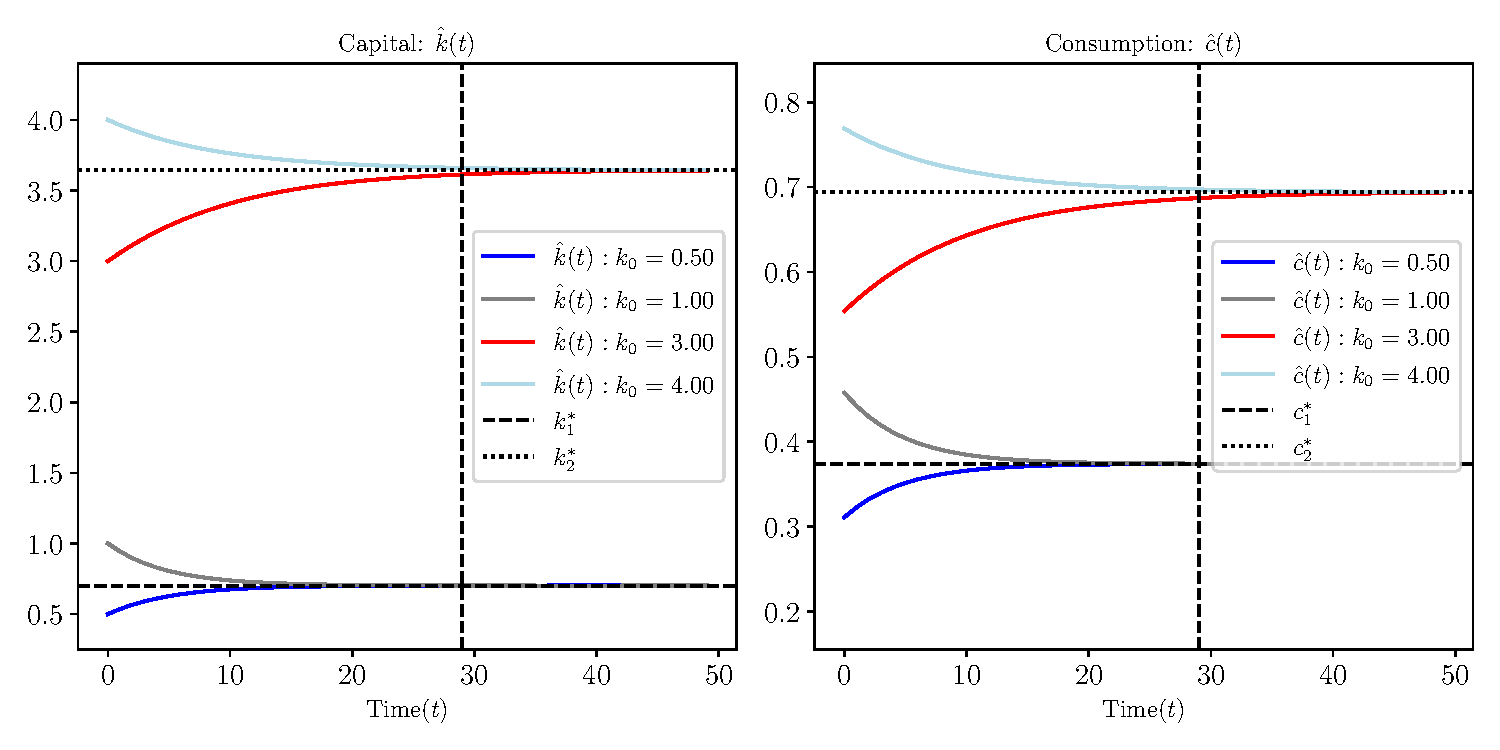
\includegraphics[width=9cm]{./figures/growth_multiple_steady_states_four_initial_k_0.pdf}
	\end{figure}
	
	\begin{enumerate}
		%\item Relative Error: $\frac{p(t)-p^f(t)}{p^f(t)}$.  Extrapolation is $t > 30 = \max_t \Xtrain$
		\item \emphcolor{Pick} $\Xtrain =\{0,\ldots,30\}$, $\alpha=\frac{1}{3}$, $\sigma =1$, $\beta = 0.9$, $g = 0.0$, $a= 0.5$, $b_1 = 3$, $b_2 = 2.5$ and $k_0 \in\{0.5,1.0,3.0,4.0\}$
		\item \emphcolor{Choose} $k(t;\theta) = NN(t;\theta)$ where ``NN'' has $4$ hidden layers of $128$ nodes. $|\Theta| = 49.9 K$ coefficients.
		\item \emphcolor{Fit} using Adam optimizer.
	\end{enumerate}
\end{frame}




\begin{frame}[label = ncg_multi_results]{Results: different initial conditions}
	
	\begin{minipage}[t]{0.4\textwidth}
		\raisebox{-\height+0.7\baselineskip}{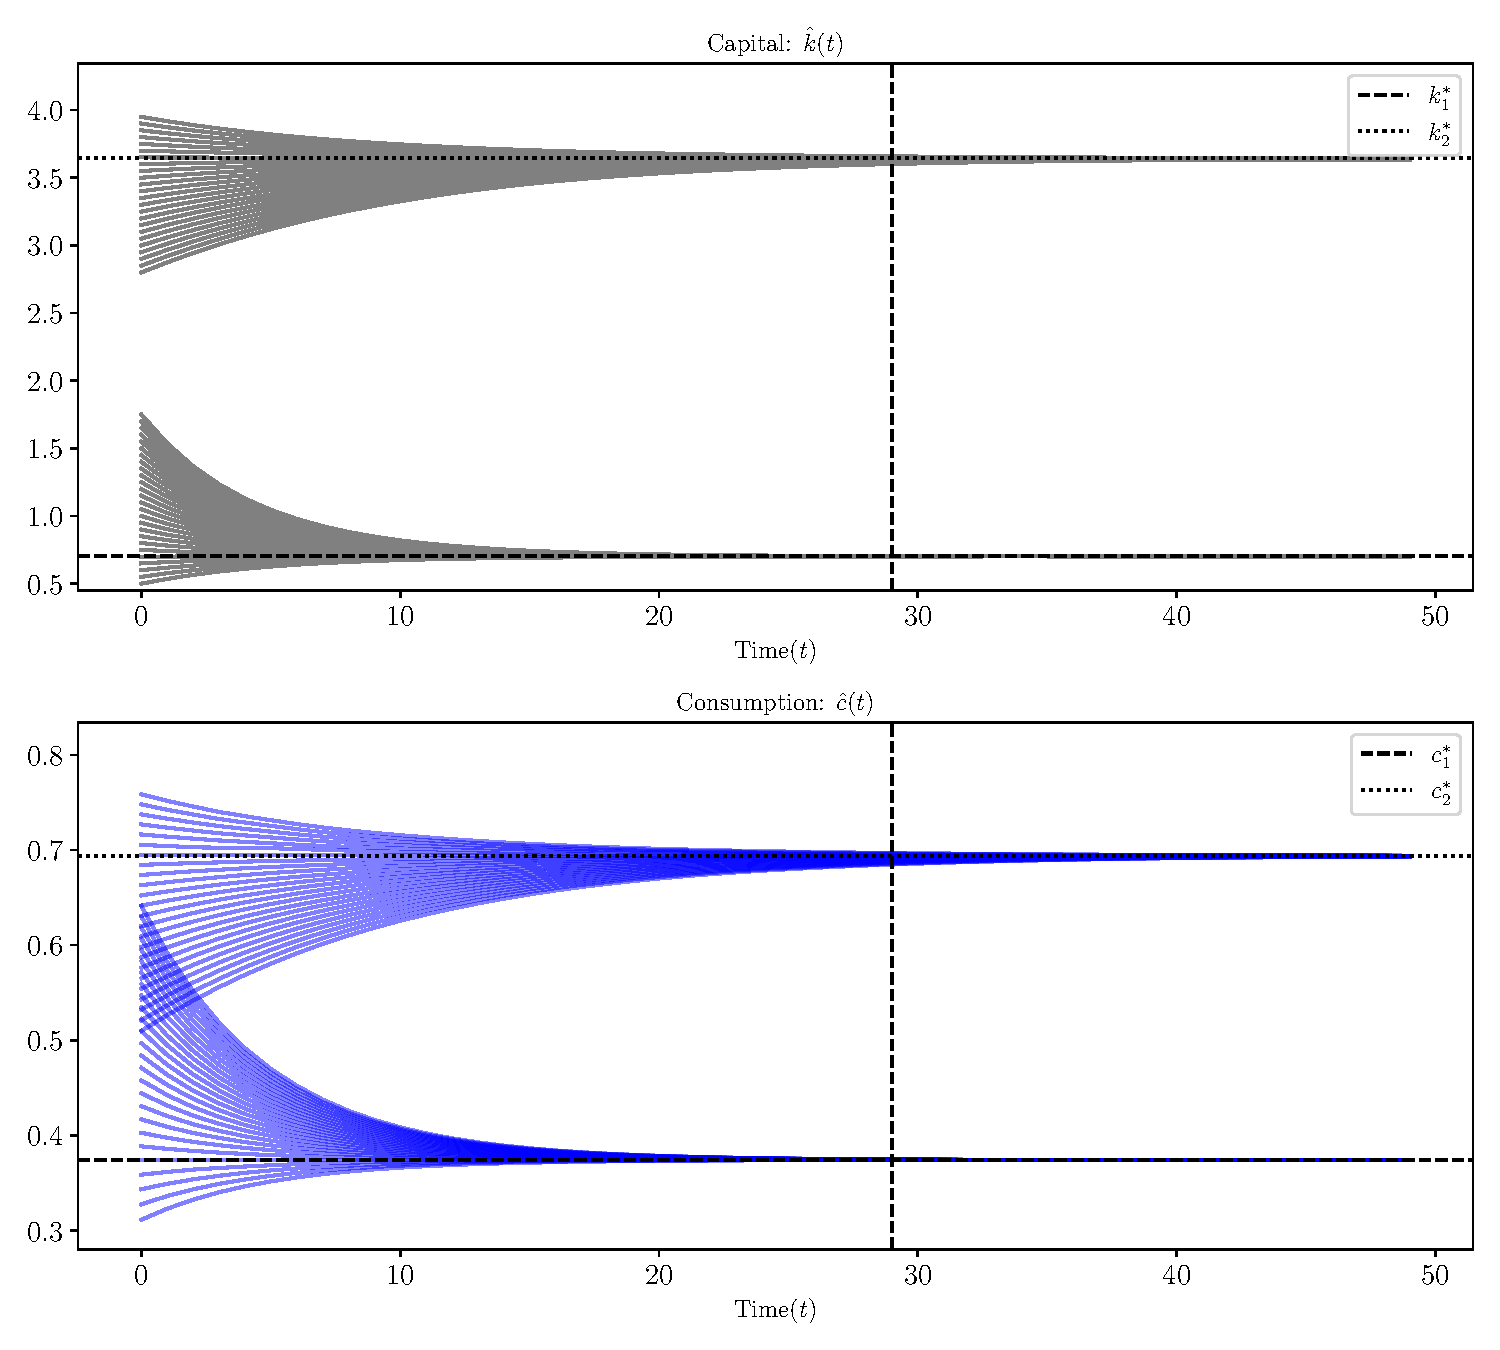
\includegraphics[width= 8cm]{./figures/growth_multiple_steady_states_var_initial_k_0.pdf}}
	\end{minipage}
	\hfill%
	\begin{minipage}[t]{0.5\textwidth}\raggedleft
		\begin{itemize}
			\item Different initial conditions in $k_0 \in [0.5,1.75]\cup[2.75,4]$.
			\smallskip
			\item In the vicinity of $k_1^*$ and $k_2^*$ the paths converge to the right steady-states.			\smallskip
			\begin{itemize}
				\item The implicit bias picks up the right path.
			\end{itemize}
			\smallskip
			\item Low generalization errors, even without imposing the transversality condition.
		\end{itemize}
	\end{minipage}
\end{frame}

\begin{frame}{Conclusion}
	
	\begin{itemize}
		\item Solving functional equations with deep learning is an extension of collocation/interpolation methods.\vspace{0.1in}
		\item With \emphcolor{massive over-parameterization}, optimizers tend to choose those interpolating functions which are not explosive and with smaller gradients (i.e., \emphcolor{inductive bias}).\vspace{0.1in}
		\item Over-parameterized solutions \emphcolor{automatically} fulfill \emphcolor{forward-looking} boundary conditions:			\smallskip
		\begin{itemize}
			\item Shedding light on the convergence of deep learning based solutions in dynamic problems in macroeconomics.	
		\end{itemize}\vspace{0.1in}
		
		\item If we solve models with deep-learning without (directly) imposing long-run boundary conditions,			\smallskip
		\begin{itemize}
			\item Short/medium-run errors are small, and long-run errors after \emphcolor{``we are all dead''} are even manageable.\smallskip
			\item Long-run errors do not affect transition dynamics even in the presence  of \emphcolor{non-stationarity} and \emphcolor{steady-state multiplicity}.			\smallskip
			\item Gives hope for solving high-dimensional models still disciplined by forward-looking economic assumptions.
		\end{itemize}\vspace{0.1in}
		
		% \begin{itemize}
			%    \item Gives hope for solving high-dimensional models still disciplined by forward looking economic assumptions.\smallskip
			%   \item With ML frameworks (e.g., PyTorch) these methods are robust \& easier to implement than alternatives.
			%\end{itemize}
		\end{itemize}
		
	\end{frame}



%\begin{frame}{Answering the challenging questions}
%	\begin{itemize}
%		\item Answering \emphcolor{generalization puzzle}: Flat  interpolation leads to good generalization:\vspace{0.1in}
%		\begin{itemize}
%			\item If the true underlying functions is flat between (and outside) the points.\vspace{0.1in}
%			\item The cure to over-fitting is to add more parameters.\vspace{0.1in}
%		\end{itemize}
%	 \item Answering \emphcolor{multiplicity puzzle}: In the linear set-up, the explosive solution has larger derivatives (less flat) than the non-explosive one i.e, $|H_1^+| > |H_1^-|$:\vspace{0.1in}
%	 \begin{itemize}
%	 	\item The deep-learning based solution \emphcolor{automatically} satisfies stationarity. \vspace{0.1in}
%	 \end{itemize}
%	\item \textcolor{red}{Ebrahimi Kahou et al. (2022)} explore this for many more dynamic models in macroeconomics (e.g., neoclassical growth and asset pricing) we show: \vspace{0.1in}
%	\begin{itemize}
%		\item We can have short- and medium-run accurate solutions without being worried about the long-run behavior.\vspace{0.1in}
%		\item  We dont need to calculate the steady-state (ergodic distribution).
%	\end{itemize} 	
%	\end{itemize}
	
%\end{frame}				

		




\section{Appendix}



\begin{frame}
	\begin{definition}[Bounded functions in $N$]
		Let:
		\begin{align*}
			\mathcal{L}(M) \equiv \{y \in \mathbb{R}^N: |y_i|\leq M ~\forall i = 1,\dots,N\}
		\end{align*}
	be an $N$-dimensional hypercube in $\mathbb{R}^N$. A function $f: \mathbb{R}^N\rightarrow \mathbb{R}$ is bounded in $N$ if for every $M$ there exists $K_M$ such that 
	\begin{equation*}
		\sup_{y\in \mathcal{L}(M)} |f(y)| < K_M,
	\end{equation*}
	where $K_M$ is a constant that does not depend on $N$, but may depend on $M$.
	\end{definition}
\begin{itemize}
	\item Example $f(y) = \frac{1}{N}\sum_{i=1}^N y_i$ $\rightarrow$ $\sup_{y\in \mathcal{L}(M)} |f(y)| < M$.\vspace{0.1in}
	\item To avoid $f(y) = \sum_{i=1}^N y_i$ $\rightarrow$ $\sup_{y\in \mathcal{L}(M)} |f(y)| < NM$.
\end{itemize}
\hyperlink{concentration}{\beamerskipbutton{back}}
\end{frame}

\begin{frame}[label = errors]
	\frametitle{Concentration of measure is the bless of dimensionality}
	In the linear case we know the closed form solution for $u$
	\begin{empheq}[box=\tcbhighmath]{align*}
		\hat{\varepsilon}\left(X;u\right)- 0 \sim \mathcal{N} \left(0,\frac{\sigma_\varepsilon^2}{N}\right)\\
		u(\hat{X}')- \condexpec{u(X')}{\omega} \sim \mathcal{N} \left(0,\frac{\sigma_u^2}{N}\right)
	\end{empheq}
	\begin{itemize}
		\item Conditional expectation becomes constant as $N$ gets large.\vspace{0.1in}
		\begin{itemize}
			\item One \emphcolor{single Monte-carlo draw} of the idiosyncratic shocks is enough.\vspace{0.1in}
			\end{itemize}
	\end{itemize}
\hyperlink{algo}{\beamerskipbutton{back}}
\end{frame}

\begin{frame}{Analytic euler error due to the concentration of measure}
	
	\begin{figure}[h!]
		\centering
		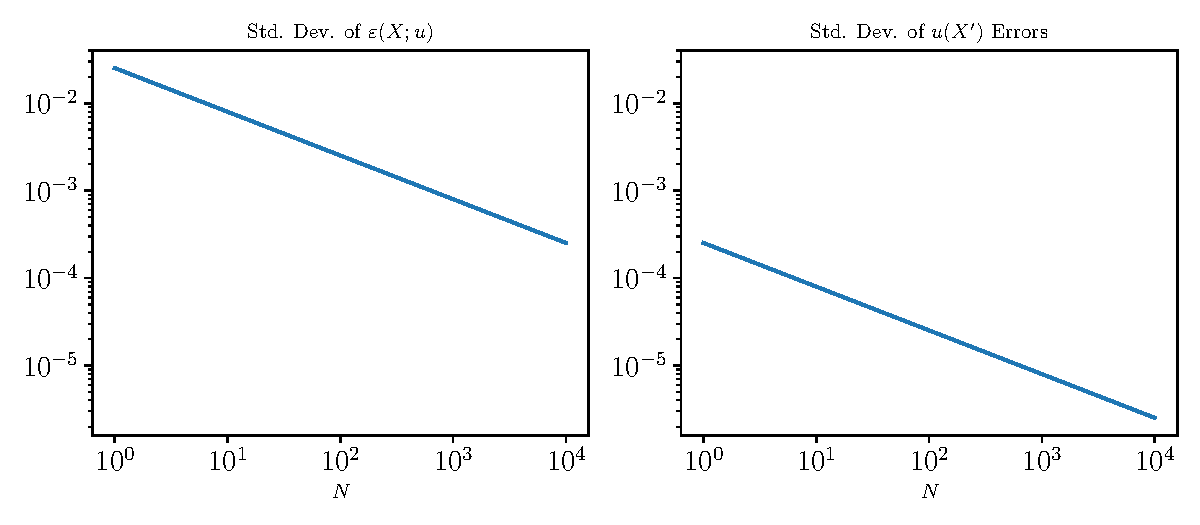
\includegraphics[height = 2.1in]{./figures/concentration_euler_residual_linear.pdf}
	\end{figure}
\end{frame}		





\begin{frame}{Parameters}
	\begin{itemize}
		\item $\gamma = 90$, $\beta = 0.95$, $\sigma = 0.005$, $\eta = 0.001$.
	\end{itemize}
\end{frame}

\begin{frame}{Implicit bias: More details}
	\label{sobolev}
	Let $\psi_1$ and $\psi_2$ be two differentiable function from a compact space $\mathcal{X}$ in $\mathbb{R}$ to $\mathbb{R}$ such that
	\begin{align*}
		\int_\mathcal{X}\left|\frac{d \psi_1}{dx}\right|^2 dx >   \int_\mathcal{X}\left|\frac{d \psi_2}{dx}\right|^2 dx
	\end{align*}
	then
	\begin{align*}
		\|\psi_1\|_S > \|\psi_2\|_S.
	\end{align*}
	%Moreover, since $\|\cdot\|_S$ is a semi-norm, it satisfies the triangle inequality
	%\begin{align}
	%	\|\psi_1+\psi_2\|_S \leq \|\psi_1\|_S + \|\psi_2\|_S.
	%\end{align}
	Recently shown the optimizers (first order e.g. SGD) regularize Sobolev semi-norms: \textcolor{red}{Ma, Ying (2021)}.
\hyperlink{implicit}{\beamerskipbutton{Back}}
\end{frame}

\end{document}
